\documentclass[12pt,fleqn]{book}

\usepackage{titlesec}
\usepackage{caption}

\titleformat{\chapter}[display]
  {\normalfont\huge\bfseries}{}{0pt}{\Huge}
\titlespacing{\chapter}
  {0pt}{10pt}{40pt}

	\newenvironment{amatrix}[1]{%
	  \left[\begin{array}{@{}*{#1}{r}|r@{}}
	}{%
	  \end{array}\right]
	}


\usepackage{amsmath,amssymb,amsfonts,graphicx,tasks,tikz,pgfplots}
\usetikzlibrary{arrows}
\pgfplotsset{compat=1.17}

\usepackage{tasks}
\settasks{
  label-width = 18pt
}
 
\makeatletter
 \def\@textbottom{\vskip \z@ \@plus 1pt}
 \let\@texttop\relax
\makeatother

\usepackage[letterpaper,margin=0.5in,footskip=.5cm]{geometry}

\setlength\parindent{0pt}

\usepackage{amsmath,amssymb,amsfonts,graphicx,tasks,tikz,pgfplots}
\usepackage{amsthm,thmtools}
\usetikzlibrary{arrows,quotes,arrows.meta,fit,shapes.geometric}

\usepackage{array}
\newcommand{\PreserveBackslash}[1]{\let\temp=\\#1\let\\=\temp}
\newcolumntype{C}[1]{>{\PreserveBackslash\centering}p{#1}}
\newcolumntype{R}[1]{>{\PreserveBackslash\raggedleft}p{#1}}
\newcolumntype{L}[1]{>{\PreserveBackslash\raggedright}p{#1}}
% Mapping diagram: one big ellipse per side, no titles
% #1 = domain elements (comma-separated)
% #2 = codomain elements (comma-separated)
% #3 = arrows as pairs i/j (i=index in domain, j=index in codomain)
% Optional keys: [xsep=5, vsep=1.2]
\newcommand{\mappingdiagram}[4][]{%
  % defaults + user overrides
  \def\xsep{5}\def\vsep{1.2}
  \tikzset{md/.cd, xsep/.store in=\xsep, vsep/.store in=\vsep}
  \tikzset{md/.cd, #1}

  \begin{tikzpicture}[>=Stealth, every node/.style={font=\large}]
    % --- Domain nodes ---
    \def\Dnodes{}%
    \foreach \d [count=\i] in {#2} {%
      \node (D\i) at (0,-\i*\vsep) {$\d$};
      \xdef\Dnodes{\Dnodes (D\i)}%
    }

    % --- Codomain nodes ---
    \def\Cnodes{}%
    \foreach \c [count=\j] in {#3} {%
      \node (C\j) at (\xsep,-\j*\vsep) {$\c$};
      \xdef\Cnodes{\Cnodes (C\j)}%
    }

    % --- Ellipses around sets ---
    \node[draw, ellipse, fit=\Dnodes, inner sep=10pt] {};
    \node[draw, ellipse, fit=\Cnodes, inner sep=10pt] {};

    % --- Arrows (i/j pairs) ---
    \foreach \a/\b in {#4} {%
      \draw[->, thick] (D\a.east) -- (C\b.west);
    }
  \end{tikzpicture}%
}


% Two-branch graph with equal scale and only max tick labels
% #1 = y1(x), #2 = y2(x), #3 = xmin, #4 = xmax, #5 = ymin, #6 = ymax,
% #7 = tick distance (ignored for equal scale), #8 = extra axis opts, #9 = plot opts
\newcommand{\graphpair}[9]{%
\begin{tikzpicture}[baseline=(current bounding box.north)]
  \begin{axis}[
    axis lines=middle,
    axis line style={very thick},
    grid style={thin,densely dotted,black!50},
    grid=major,
    xmin=#3-.2, xmax=#4+.2,
    ymin=#5-.2, ymax=#6+.2,
    xlabel=$x$, ylabel=$y$,
    axis equal image,
    % Only show largest tick values on each axis
    xticklabels={},
	yticklabels={},
	xtick distance=1, ytick distance=1,
	extra x ticks={#4},
	extra y ticks={#6},
    enlargelimits=false,
    % Allow optional extra axis settings
    #8
  ]
    \addplot[domain=#3:#4, samples=500, #9] (x,{#1});
    \addplot[domain=#3:#4, samples=500, #9] (x,{#2});
  \end{axis}
\end{tikzpicture}%
}


\newcommand{\graph}[8]{
\begin{tikzpicture}[baseline=(current bounding box.north)]
  \begin{axis}[
    axis lines=middle,
    axis line style={very thick},
    grid style={thin,densely dotted,black!50},
    grid=major,
      xtick distance=#6, ytick distance=#6,
      xmin=#2-.2, xmax=#3+.2,
      ymin=#4-.2, ymax=#5+.2,
      xlabel=$x$,
      ylabel=$y$,
    xticklabels={},
	yticklabels={},
	xtick distance=1, ytick distance=1,
	extra x ticks={#3},
	extra y ticks={#5},
      #7]
      \addplot[
      domain=#2:#3,
      samples=500,#8]
      (x,{#1});
    \end{axis}
  \end{tikzpicture}
}

\newcommand{\graphtwo}[9]{
\begin{tikzpicture}[baseline=(current bounding box.north)]
  \begin{axis}[
    axis lines=middle,
    axis line style={very thick},
    grid style={thin,densely dotted,black!50},
    grid=major,
      xtick distance=#7, ytick distance=#7,
\usepackage{amsmath,amssymb,amsfonts,amsthm,thmtools}
      xmin=#3-.2, xmax=#4+.2,
      ymin=#5-.2, ymax=#6+.2,
      xlabel=$x$,
      ylabel=$y$,
      #8]
      \addplot[
      domain=#3:#4,
      samples=500,#9]
      (x,{#1});
      \addplot[
      domain=#3:#4,
      samples=500,#9]
      (x,{#2});
    \end{axis}
  \end{tikzpicture}
}

\newcommand{\curve}[7]{% function, xmin, xmax, ymin, ymax, 
\begin{tikzpicture}[baseline=(current bounding box.north)]
  \begin{axis}[
    axis lines=middle,
    axis line style={very thick},
    grid style={thin,densely dotted,black!50},
    grid=major,
    xticklabels={},
	yticklabels={},
	xtick distance=1, ytick distance=1,
	extra x ticks={#3},
	extra y ticks={#5},
      xmin=#2-.2, xmax=#3+.2,
      ymin=#4-.2, ymax=#5+.2,
      xlabel=$x$,
      ylabel=$y$,
      #6]
      \addplot[
      domain=#2:#3,
      samples=500,#7]
      (x,{#1});
    \end{axis}
  \end{tikzpicture}
}

\newcommand{\blankgraph}[6]{
\begin{tikzpicture}[baseline=(current bounding box.north)]
  \begin{axis}[
    width=#5in,height=#6in,
    axis lines=middle,
    axis line style={very thick},
    grid style={thin,densely dotted,black!50},
    grid=major,
    xticklabels={},
	yticklabels={},
	xtick distance=1, ytick distance=1,
	extra x ticks={#2},
	extra y ticks={#4},
      xtick distance=1, ytick distance=1,
      xticklabels={1},
      yticklabels={1},
      xmin=#1-.2, xmax=#2+.2,
      ymin=#3-.2, ymax=#4+.2,
      xlabel=$x$,
      ylabel=$y$]
    \end{axis}
  \end{tikzpicture}
}

\newcommand{\blankaxes}[2]{
\begin{tikzpicture}[baseline=(current bounding box.north)]
  \begin{axis}[
    width=#1in,height=#2in,
    axis lines=middle,
    axis line style={very thick},
    grid=major,
    xtick distance=2, ytick distance=2,
    xmin=-1, xmax=1,
    ymin=-1, ymax=1,
    xlabel=$x$,
    ylabel=$y$]
  \end{axis}
\end{tikzpicture}
}

\newcommand{\ds}{\displaystyle}

\newcommand{\lr}[1]{\left(#1\right)}

% \usepackage{amsthm}
% \theoremstyle{definition}
% \newtheorem{problem}{}
% \counterwithin*{problem}{section}
% \renewcommand{\theproblem}{\thesubsection.\arabic{problem}}
%
% \newtheorem*{solutionx}{\thesolutionnumber}
% \ExplSyntaxOn
% \tl_new:N \g_gargantuar_solution_tl
%
% \NewDocumentEnvironment{solution}{+b}
%  {
%   \tl_gput_right:Nx \g_gargantuar_solution_tl
%    {
%     \printsolution{\theproblem}{ \exp_not:n { #1 } }
%    }
%  }
%  {}
% \NewDocumentCommand{\printsolutions}{}
%  {
%   \tl_use:N \g_gargantuar_solution_tl
%   \tl_gclear:N \g_gargantuar_solution_tl
%  }
% \NewDocumentCommand{\printsolution}{m +m}
%  {
%   \cs_set:Npn \thesolutionnumber { #1 }
%   \begin{solutionx} #2 \end{solutionx}
%  }
% \ExplSyntaxOff
% \makeatother
%
% \newcommand{\prb}[1]{\begin{problem}#1\end{problem}}
% \newcommand{\sol}[1]{\begin{solution}#1\end{solution}}
% =============================
% TCOLORBOX CONFIGURATION
% =============================

\usepackage{tcolorbox}

\definecolor{black}{rgb}{0,0,0}
\definecolor{dark-gray}{rgb}{.15,.15,.15}
\definecolor{light-gray}{rgb}{.85,.85,.85}
\definecolor{white}{rgb}{1,1,1}

\makeatletter
\newcommand*\ifcounter[1]{%
	\ifcsname c@#1\endcsname
		\expandafter\@firstoftwo
	\else
		\expandafter\@secondoftwo
	\fi
}
\makeatother

\tcbuselibrary{theorems}

\ifcounter{unit}{
	\newtcbtheorem{defn}{Definition \theunit.\hspace{-.3em}}{
		colback=light-gray,colframe=dark-gray,coltitle=white,coltext=black,fonttitle=\bfseries,before skip=20pt plus 2pt,after skip=20pt plus 2pt}{th}
}{
	\newtcbtheorem{defn}{Definition}{
		colback=light-gray,colframe=dark-gray,coltitle=white,coltext=black,fonttitle=\bfseries,before skip=20pt plus 2pt,after skip=20pt plus 2pt}{th}
}

\ifcounter{unit}{
	\newtcbtheorem{thm}{Theorem \theunit.\hspace{-.3em}}{
		colback=light-gray,colframe=dark-gray,coltitle=white,coltext=black,fonttitle=\bfseries,before skip=20pt plus 2pt,after skip=20pt plus 2pt}{th}
}{
	\newtcbtheorem{thm}{Theorem}{
		colback=light-gray,colframe=dark-gray,coltitle=white,coltext=black,fonttitle=\bfseries,before skip=20pt plus 2pt,after skip=20pt plus 2pt}{th}
}



\pagestyle{plain}
\usepackage[lastexercise,answerdelayed]{exercise}
\usepackage{totcount}
\regtotcounter{Exercise} % register the counter for getting the total
\usepackage{chngcntr}
\counterwithin{Exercise}{chapter}
\counterwithin{Answer}{chapter}
\usepackage{xassoccnt}
\NewTotalDocumentCounter{totalex}
\usepackage{titleref}
\usepackage{etoolbox}

%EXERCISE START

\renewcommand{\ExerciseHeader}{ \stepcounter{totalex}\ifnumcomp{\value{Exercise}}{=}{1}{\ifnumcomp{\thechapter}{=}{1}{}{\vspace{10pt}}\noindent\Large\textbf{Exercises}\par\vspace{10pt}}{}\noindent\normalsize\bfseries\ExerciseHeaderNB\ExerciseHeaderDifficulty.}
\renewcommand{\AnswerHeader}{\ifnumcomp{\value{Exercise}}{=}{1}{\ifnumcomp{\thechapter}{=}{1}{}{\vspace{10pt}}\noindent\Large\textbf{Section\ \thechapter\ Solutions}\par\vspace{10pt}}{}\noindent\normalsize\bfseries\ExerciseHeaderNB.\ }

\usepackage{hyperref}

\newcommand{\prb}[1]{\begin{Exercise}#1\end{Exercise}}
\newcommand{\sol}[1]{\begin{Answer}#1\end{Answer}}

%EXERCISE END



\begin{document}
\noindent
\thispagestyle{empty}
Grade 10 Advanced Math \hfill Name: \hspace{2in}
\medskip\hrule
\noindent

\vfill

\begin{center}
	{\bf \huge Chapter 2: Quadratic Functions}
\end{center}

\vfill
\vfill

\clearpage

\setcounter{page}{1}

{\bf \huge Introduction }
\\[2em]
When a function is linear, as the independent variable increases, the dependent variable increases by the same amount.  In other words, a linear function has a slope that remains constant.
\\[1em]
The next kind of function we will learn about is a special type of non-linear function.  This function will have different slopes at different areas, meaning it will grow faster at some places than others.
\\[1em]
Consider the two visual patterns below:
\\[3in]
Make a difference table for each visual pattern.  What do you notice?  Can you make a difference table of differences?
\\[1em]
A function is quadratic when its slope grows linearly.  Some examples of quadratic functions are:
\begin{align*}
	y & =x^2                                                      \\
	y & =x^2+5                                                    \\
	y & =\frac 12 x^2                                             \\
	y & =2x^2 - x + 1                                             \\
	y & =ax^2 + bx + c \quad\quad\quad a,b,c\in \mathbb R, a\ne 0 \\
\end{align*}
What do you notice about these quadratic functions?\\[1in]
Write some examples of quadratic functions.
\clearpage
\chapter{1. Graphing Quadratic Functions.}
Graphing quadratic functions is similar to graphing linear functions but requires a little more care, and in some cases more algebra.
\\[1em]
To see this, let's start by using a table of values to help us make a graph.  We'll start with the most basic quadratic function: $y=x^2.$  Write a table of values that include $x=-3,-2,-1,0,1,2,3$ on the left, and the corresponding y value on the right.  When you're done, plot those points on the graph given to you.
\[
	\blankgraph{-10}{10}{-10}{10}{4}{4}
\]
The name of this shape is a {\bf parabola}.  Just like a rectangle or a triangle, a parabola can take many forms.  As the function changes, the shape changes along with it.  For example, $y=x^2$ looks very different from $y=-\frac{1}{8}x^2-3x+7$.
\\[1em]
Make a few notes about the shape you see from the parabola you graphed.
\vfill
Question: is the tip of a parabola pointy?
\clearpage
Use a table of values using the following values: $0,\ 0.1,\ 0.2,\ 0.3,\ \ldots,\ 0.9,\ 1.0$.  When you're finished, try to connect the dots as smoothly as possible.
\[
	\blankgraph{0}{11}{0}{11}{5}{5}
\]
Draw a small parabola to the best of your abilities using the space below.
\\[1.5in]
Draw three more parabolas: one with no $x$-intercepts, the second with exactly one $x$-intercept, and a third with exactly two $x$-intercepts.  Label every $x$-intercept that there is.
\[
	\blankaxes{2.5}{2.5}\hfill
	\blankaxes{2.5}{2.5}\hfill
	\blankaxes{2.5}{2.5}
\]
In each of these scenarios, how many $y$-intercepts did the parabola have?  Label each one.
\clearpage
Sometimes parabolas point upward, sometimes they point downwards.  When they point upwards, both ends of the parabola point up, and when they point downwards, both tips point down.  Draw a parabola that has two $x$-intercepts, and points downwards.
\[
	\blankaxes{2.5}{2.5}
\]
When a parabola points upwards, it has a minimum point: a point that has a $y$-value that is less than any other point.  Similarly, when a parabola points downwards, it has a maximum point.  In both scenarios, we call that point the {\bf vertex}.
\\[1em]
Go back to all the parabolas you have made and circle the vertex and label it ``vertex''.
\\[1em]
You may have noticed that parabolas are symmetric.  They are symmetric around a particular vertical line.  This line is called the {\bf axis of symmetry}.  Go back to all the parabolas you have made and draw a dashed line along the axis of symmetry and label it ``axis of symmetry''.  When you're done, all of your parabolas should look something like this:
\[
	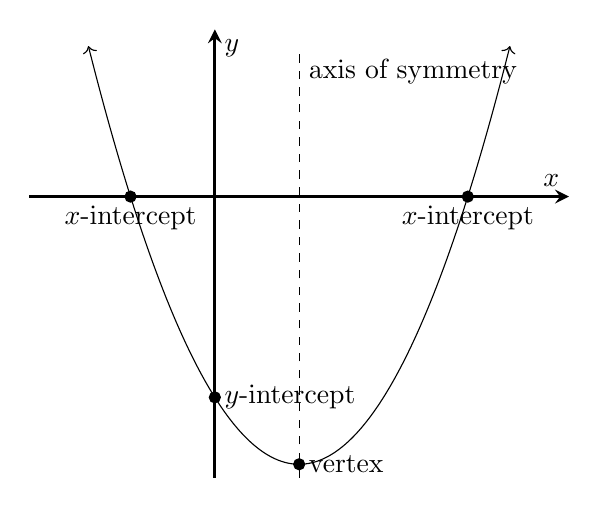
\begin{tikzpicture}[baseline=(current bounding box.north)]
		\begin{axis}[
				axis lines=middle,
				axis line style={very thick},
				grid style={thin,densely dotted,black!50},
				grid=major,
				xtick distance=5, ytick distance=5,
				xmin=-2-.2, xmax=4+.2,
				ymin=-4-.2, ymax=2+.5,
				xlabel=$x$,
				ylabel=$y$]
			\draw [dashed] (1,-4.2) -- (1,2.2) node[anchor=north west]{axis of symmetry};
			\filldraw[black] (-1,0) circle (2pt) node[anchor=north]{$x$-intercept};
			\filldraw[black] (3,0) circle (2pt) node[anchor=north]{$x$-intercept};
			\filldraw[black] (1,-4) circle (2pt) node[anchor=west]{vertex};
			\filldraw[black] (0,-3) circle (2pt) node[anchor=west]{$y$-intercept};
			\addplot[
				domain=-1.5:3.5,
				samples=500,<->]
			(x,{(x-1)^2-4});
		\end{axis}
	\end{tikzpicture}
\]
The domain of a quadratic function is all real numbers, every time.  That means $x$ will take on every possible number in a quadratic function.  Think: which numbers $x$ can I square to make $x^2$?
\\[1em]
The range of a quadratic function depends on a few things.  First, it depends on the $y$-value of the vertex.  It also depends on the direction the parabola is pointing.  Is it pointing upwards or downwards?  If it's pointing upwards, then the vertex represents a minimum value, and all other $y$-values on the vertex must be greater than the $y$-value of the vertex.  The same thing, except opposite, can be said if the parabola is pointing downwards.
\clearpage
Consider the parabola below.
\[
	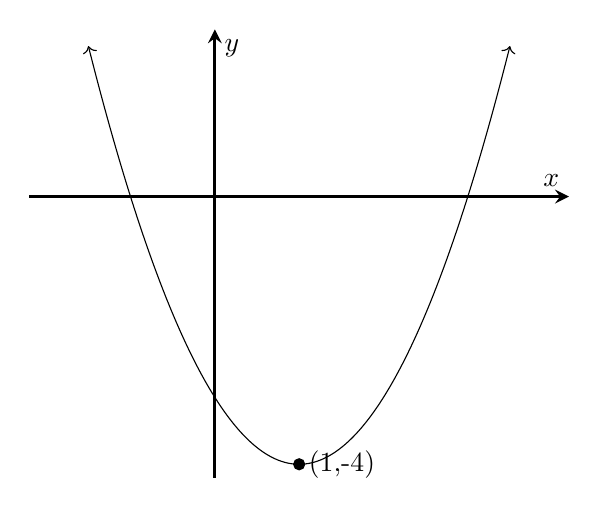
\begin{tikzpicture}[baseline=(current bounding box.north)]
		\begin{axis}[
				axis lines=middle,
				axis line style={very thick},
				grid style={thin,densely dotted,black!50},
				grid=major,
				xtick distance=5, ytick distance=5,
				xmin=-2-.2, xmax=4+.2,
				ymin=-4-.2, ymax=2+.5,
				xlabel=$x$,
				ylabel=$y$]
			\filldraw[black] (1,-4) circle (2pt) node[anchor=west]{(1,-4)};
			\addplot[
				domain=-1.5:3.5,
				samples=500,<->]
			(x,{(x-1)^2-4});
		\end{axis}
	\end{tikzpicture}
\]
As you can see, the parabola does not have any points that have $y$-coordinates less than 4.  That's because it points upwards, and the vertext is at the point $(1,4)$.

But for any value of $y$ greater than or equal to $-4$ there is at least one point on the parabola that has that value.  So the range includes all values of $y$ greater than or equal to $-4$.  We can write this in several ways:
\begin{itemize}
	\item $y\ge -4$
	\item $[-4,\infty)$
	\item $\{y\in \mathbb R : y \ge 4\}$
\end{itemize}
However you choose to express the range is up to you, but you should double check with your teacher that your notation is consistent.
\prb{Give an example of a quadratic function.}\vspace{4em}
\sol{There are infinitely many quadratic functions, but one could be $y=2x^2-\pi x + \sqrt{18}$}
\prb{If a parabola opens upwards, is the vertex a maximum or a minimum?}\vspace{4em}
\sol{The vertex is a minimum when the parabola points upwards.}
\prb{A quadratic function is a polynomial of what degree?}
\vspace{4em}
\sol{A quadratic function is a degree 2 polynomial.}
\clearpage
\prb{Identify the direction of opening, $x$-intercepts, $y$-intercept, vertex, and axis of symmetry in each quadratic function given.
	\begin{tasks}(2)
		\task
		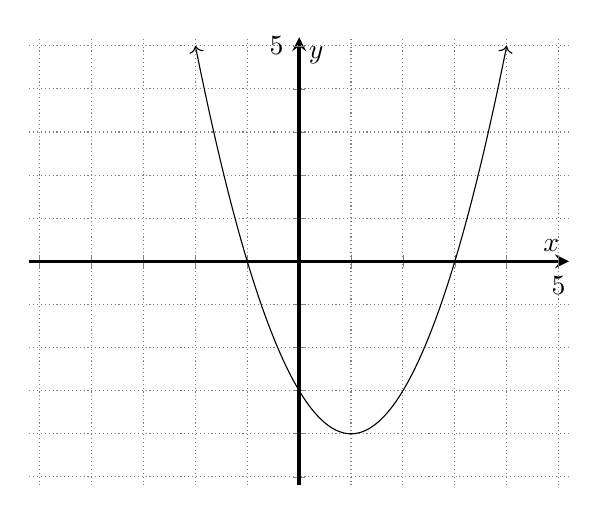
\begin{tikzpicture}[baseline=(current bounding box.north)]
			\begin{axis}[
					xticklabels={},
					yticklabels={},
					extra x ticks={5},
					extra y ticks={5},
					axis lines=middle,
					axis line style={very thick},
					grid style={thin,densely dotted,black!50},
					grid=major,
					xtick distance=1, ytick distance=1,
					xmin=-5-.2, xmax=5+.2,
					ymin=-5-.2, ymax=5+.2,
					xlabel=$x$,
					ylabel=$y$]
				\addplot[
					domain=-2:4,
					samples=500,<->]
				(x,{(x-1)^2-4});
			\end{axis}
		\end{tikzpicture}
		\vspace{2in}
		\task
		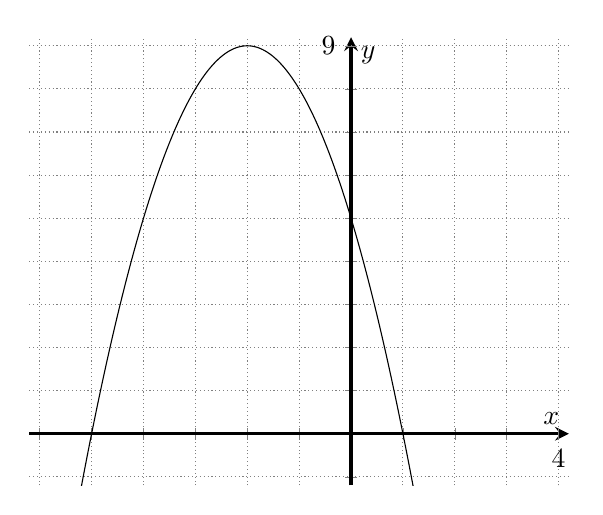
\begin{tikzpicture}[baseline=(current bounding box.north)]
			\begin{axis}[
					xticklabels={},
					yticklabels={},
					extra x ticks={4},
					extra y ticks={9},
					axis lines=middle,
					axis line style={very thick},
					grid style={thin,densely dotted,black!50},
					grid=major,
					xtick distance=1, ytick distance=1,
					xmin=-6-.2, xmax=4+.2,
					ymin=-1-.2, ymax=9+.2,
					xlabel=$x$,
					ylabel=$y$]
				\addplot[
					domain=-6:5,
					samples=500,<->]
				(x,{-(x+2)^2+9});
			\end{axis}
		\end{tikzpicture}
		\task
		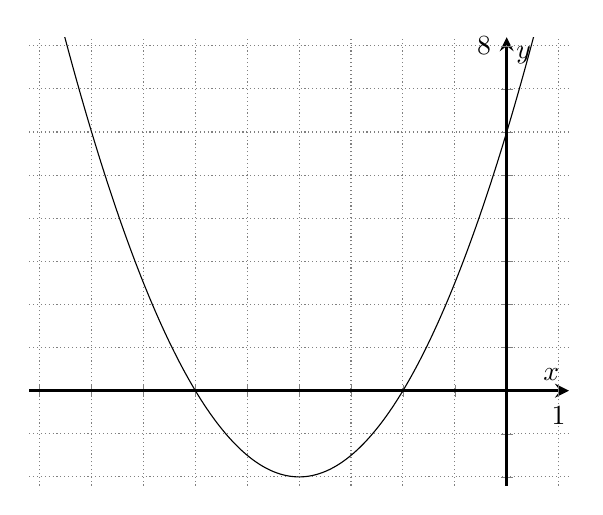
\begin{tikzpicture}[baseline=(current bounding box.north)]
			\begin{axis}[
					xticklabels={},
					yticklabels={},
					extra x ticks={1},
					extra y ticks={8},
					axis lines=middle,
					axis line style={very thick},
					grid style={thin,densely dotted,black!50},
					grid=major,
					xtick distance=1, ytick distance=1,
					xmin=-9-.2, xmax=1+.2,
					ymin=-2-.2, ymax=8+.2,
					xlabel=$x$,
					ylabel=$y$]
				\addplot[
					domain=-9:1,
					samples=500,<->]
				(x,{1/2*(x+4)^2-2});
			\end{axis}
		\end{tikzpicture}
		\task
		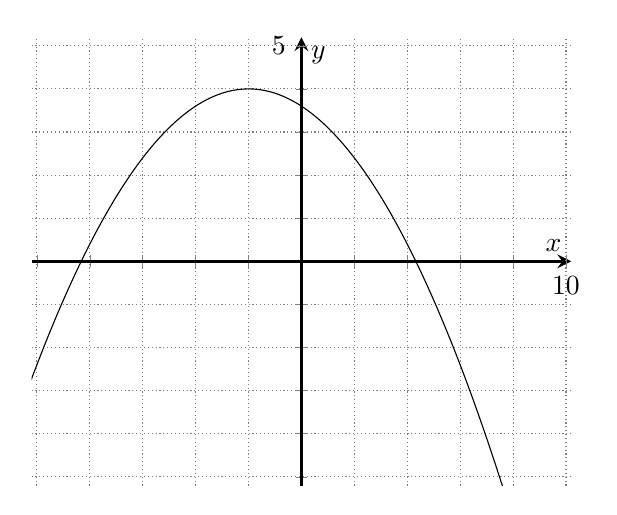
\begin{tikzpicture}[baseline=(current bounding box.north)]
			\begin{axis}[
					xticklabels={},
					yticklabels={},
					extra x ticks={10},
					extra y ticks={5},
					axis lines=middle,
					axis line style={very thick},
					grid style={thin,densely dotted,black!50},
					grid=major,
					xtick distance=2, ytick distance=1,
					xmin=-10-.2, xmax=10+.2,
					ymin=-5-.2, ymax=5+.2,
					xlabel=$x$,
					ylabel=$y$]
				\addplot[
					domain=-11:10,
					samples=500,<->]
				(x,{-0.1*(x+2)^2+4});
			\end{axis}
		\end{tikzpicture}
		\vspace{2in}
	\end{tasks}
}
\sol{
	\begin{tasks}(2)
		\task
		Opens upward.\\
		Vertex: $(1,-4).$\\
		$x$-intercepts: $(-1,0)$ and $(3,0)$.\\
		$y$-intercept: $(0,-3)$.\\
		Axis of symmetry: $x=1$.
		\task
		Opens downward.\\
		Vertex: $(-2,-9).$\\
		$x$-intercepts: $(-5,0)$ and $(1,0)$.\\
		$y$-intercept: $(0,5)$.\\
		Axis of symmetry: $x=-2$.
		\task
		Opens upward.\\
		Vertex: $(-4,-2).$\\
		$x$-intercepts: $(-6,0)$ and $(-2,0)$.\\
		$y$-intercept: $(0,6)$.\\
		Axis of symmetry: $x=-4$.
		\task
		Opens downward.\\
		Vertex: $(-1,4).$\\
		$x$-intercepts: approximately $(-8.2,0)$ and $(4.2,0)$.\\
		$y$-intercept: approximately $(0,3.5)$.\\
		Axis of symmetry: $x=-1$.
	\end{tasks}
}
\clearpage
\prb{Graph each of the following functions by using a table of values.  Then identify the vertex, axis of symmetry, and all $x$- and $y$-intercepts.
	\begin{tasks}(2)
		\task $y=x^2+x+3$
		\\[1em]\blankgraph{-3}{3}{-1}{5}{3}{3}
		\vspace{1in}
		\task $y=\frac12 x^2 -x -1$
		\\[1em]\blankgraph{-2}{4}{-2}{4}{3}{3}
		\vspace{1in}
		\task $y=(x-3)^2-1$
		\\[1em]\blankgraph{-1}{5}{-1}{5}{3}{3}
		\vspace{1in}
		\task $y=(x+2)^2-5$
		\\[1em]\blankgraph{-5}{1}{-5.5}{1}{3}{3}
	\end{tasks}
}
\prb{A quadratic function has two $x$-intercepts at $(2,0)$ and $(-3,0)$, respectively.  What is the axis of symmetry?}
\vspace{.5in}
\sol{The axis of symmetry is found exactly between the two $x$-intercepts at $x=-\frac 12$.}
\prb{A quadratic function has a vertex at $(-2,1)$ and an $x$-intercept at $(3,0)$.  Find the other $x$-intercept.}
\sol{Since the axis of symmetry passes through the vertex, the other $x$-intercept will lie on the other side of the axis of symmetry, which is at the point $(8,0)$.}
\clearpage
\chapter{2. Vertex Form}
One of the most vital components of a quadratic function is its vertex.  It is either the minimum or maximum value, and also is the only point on the graph that the axis of symmetry passes through.
\\[1em]
Maybe you remember the emphasis that your math teacher put on slope-point form.  The valuable thing about slope-point form is that you can start graphing the line anywhere - not just the $y$-axis.  The same can be said about graphing a quadratic function.  We don't often start graphing a quadratic at the $y$-axis.  Instead, we try to start graphing a quadratic function at its vertex.
\\[1em]
Just like slope-point form is a way of expressing a linear function, vertex form is a way of expressing a quadratic function.
\\[1em]
To understand vertex form, we'll start by graphing a few quadratic functions by using a table of values.
\\[1em]
First, graph $y=x^2$.  Notice the gaps between the $y$-values.  Take your time graphing this one since its the most important one.  We will base all of the subsequent graphs off of this one.
\\[1em]\blankgraph{-4}{4}{-3}{10}{3.5}{5}
\clearpage
Graph the following using a table of values.  While you are graphing them, make a note about how this graph is different than the graph of $y=x^2.$ 
\begin{tasks}(2)
	\task $y=x^2 + 3$
	\\[1em]\blankgraph{-4}{4}{-1}{12}{3.5}{5}
	\task $y=x^2 - 4$
	\\[1em]\blankgraph{-4}{4}{-5}{8}{3.5}{5}
    \\[25em]
	\task $y=(x-1)^2$
	\\[1em]\blankgraph{-3}{5}{-1}{12}{3.5}{5}
	\task $y=(x+3)^2$
	\\[1em]\blankgraph{-6}{2}{-1}{12}{3.5}{5}
	\task $y=-x^2$
	\\[1em]\blankgraph{-4}{4}{-12}{1}{3.5}{5}
	\task $y=\frac12 x^2$
	\\[1em]\blankgraph{-4}{4}{-3}{10}{3.5}{5}
	\task $y=-2x^2$
	\\[1em]\blankgraph{-4}{4}{-10}{3}{3.5}{5}
	\task $y=-\frac 12 (x-3)^2+1$
	\\[1em]\blankgraph{-6}{2}{-10}{3}{3.5}{5}
\end{tasks}
\clearpage
Recall the formula for slope-point form: $y=m(x-x_0)+y_0$.
\\[1em]
What do you think the formula for vertex form is?
\\[6em]
Using your formula, try to find the equation of the following quadratic functions:
\begin{tasks}(2)
	\task
	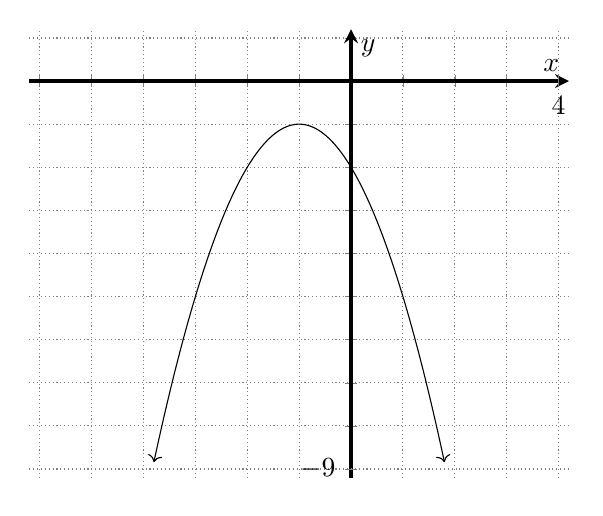
\begin{tikzpicture}[baseline=(current bounding box.north)]
		\begin{axis}[
				xticklabels={},
				yticklabels={},
				extra x ticks={4},
				extra y ticks={-9},
				axis lines=middle,
				axis line style={very thick},
				grid style={thin,densely dotted,black!50},
				grid=major,
				xtick distance=1, ytick distance=1,
				xmin=-6-.2, xmax=4+.2,
				ymin=-9-.2, ymax=1+.2,
				xlabel=$x$,
				ylabel=$y$]
			\addplot[
				domain=-3.8:1.8,
				samples=500,<->]
			(x,{-1*(x+1)^2-1});
		\end{axis}
	\end{tikzpicture}
	\task
	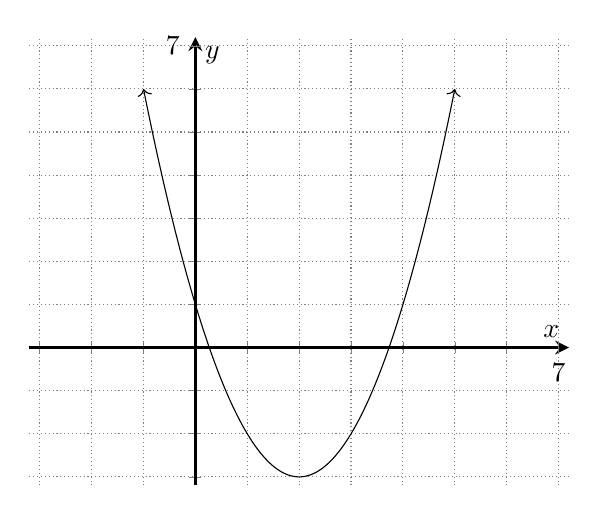
\begin{tikzpicture}[baseline=(current bounding box.north)]
		\begin{axis}[
				xticklabels={},
				yticklabels={},
				extra x ticks={7},
				extra y ticks={7},
				axis lines=middle,
				axis line style={very thick},
				grid style={thin,densely dotted,black!50},
				grid=major,
				xtick distance=1, ytick distance=1,
				xmin=-3-.2, xmax=7+.2,
				ymin=-3-.2, ymax=7+.2,
				xlabel=$x$,
				ylabel=$y$]
			\addplot[
				domain=-1:5,
				samples=500,<->]
			(x,{(x-2)^2-3});
		\end{axis}
	\end{tikzpicture}
	\\[1.5in]
	\task
	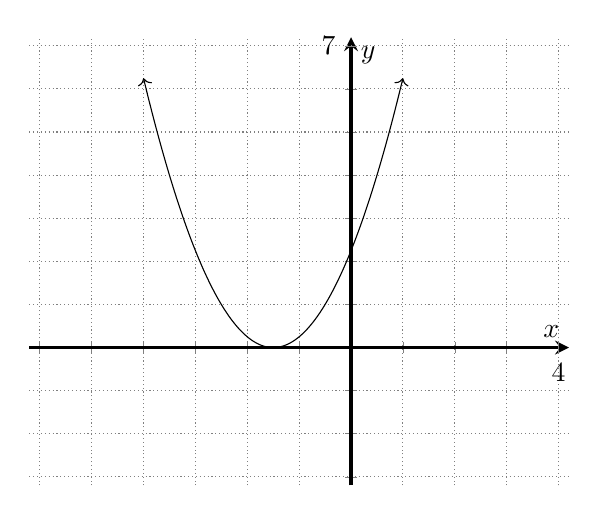
\begin{tikzpicture}[baseline=(current bounding box.north)]
		\begin{axis}[
				xticklabels={},
				yticklabels={},
				extra x ticks={4},
				extra y ticks={7},
				axis lines=middle,
				axis line style={very thick},
				grid style={thin,densely dotted,black!50},
				grid=major,
				xtick distance=1, ytick distance=1,
				xmin=-6-.2, xmax=4+.2,
				ymin=-3-.2, ymax=7+.2,
				xlabel=$x$,
				ylabel=$y$]
			\addplot[
				domain=-4:1,
				samples=500,<->]
			(x,{(x+1.5)^2});
		\end{axis}
	\end{tikzpicture}
	\task
	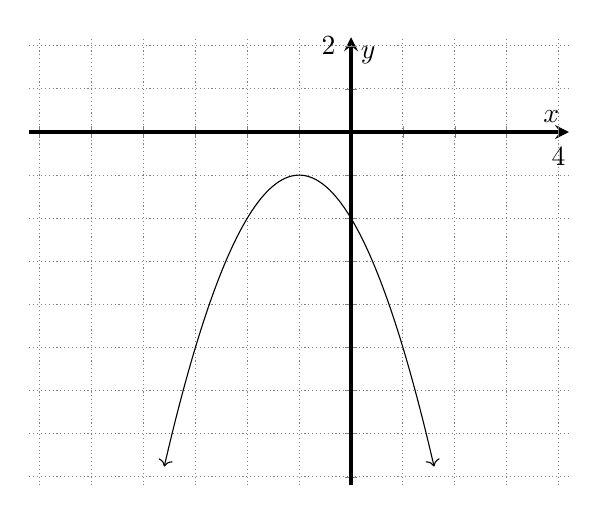
\begin{tikzpicture}[baseline=(current bounding box.north)]
		\begin{axis}[
				xticklabels={},
				yticklabels={},
				extra x ticks={4},
				extra y ticks={2},
				axis lines=middle,
				axis line style={very thick},
				grid style={thin,densely dotted,black!50},
				grid=major,
				xtick distance=1, ytick distance=1,
				xmin=-6-.2, xmax=4+.2,
				ymin=-8-.2, ymax=2+.2,
				xlabel=$x$,
				ylabel=$y$]
			\addplot[
				domain=-3.6:1.6,
				samples=500,<->]
			(x,{-(x+1)^2-1});
		\end{axis}
	\end{tikzpicture}
\end{tasks}
\clearpage
\prb{What is the formula for a quadratic function in vertex form?  Use variables $(h,k)$.}
\vspace{1in}
\sol{A quadratic function with vertex $(h,k)$ is the following:
	\[
		y=(x-h)^2+k
	\]
}
\prb{Find the quadratic function for each of the following parabolas.
	\begin{tasks}(2)
		\task
		\curve{(x-2)^2+1}{-1}{5}{-1}{5}{}{<->}
		\vspace{1in}
		\task
		\curve{(x+2)^2-3}{-5}{1}{-5}{1}{}{<->}
		\vspace{1in}
		\task
		\curve{(x+1)^2+1}{-5}{3}{-1}{7}{}{<->}
		\vspace{1in}
		\task
		\curve{(x-1)^2-2}{-2}{4}{-3}{3}{}{<->}
		\vspace{1in}
	\end{tasks}
}
\sol{
	\begin{tasks}(4)
		\task $y=(x-2)^2+1$
		\task $y=(x+2)^2-3$
		\task $y=(x+1)^2+1$
		\task $y=(x-1)^2-2$
	\end{tasks}
	\clearpage }
\clearpage
\prb{Graph the following quadratic functions.
	\begin{tasks}(2)
		\task $y=(x+1)^2-3$\\
		\blankgraph{-4}{2}{-4}{2}{3}{3}
		\task $y=(x-3)^2+1$\\
		\blankgraph{-1}{5}{-1}{5}{3}{3}
		\task $y=(x-1)^2-1$\\
		\blankgraph{-2}{4}{-2}{4}{3}{3}
		\task $y=x^2-3$\\
		\blankgraph{-3}{3}{-5}{1}{3}{3}
	\end{tasks}
}
\sol{
	\begin{tasks}(2)
		\task
		\curve{(x+1)^2-3}{-4}{2}{-4}{2}{}{<->}
		\task
		\curve{(x-3)^2+1}{-1}{5}{-1}{5}{}{<->}
		\task
		\curve{(x-1)^2-1}{-2}{4}{-2}{4}{}{<->}
		\task
		\curve{x^2-3}{-3}{3}{-5}{1}{}{<->}
	\end{tasks}
}
\prb{Without graphing, determine the number of $x$-intercepts of the function $y=(x-3)^2+1$
	\\[3em]
}
\sol{There are no $x$-intercepts because the parabola is above the $x$-axis and is pointing upwards.}
\prb{Not all quadratics have the same number of $x$-intercepts.  Is the same true about $y$-intercepts?
	\\[3em]
}
\sol{No.  All quadratics have exactly one $y$-intercept.}
\prb{Suppose $f(x)=(x-5)^2+k$ for some value $k$.  If $f(7)=19$, can you find $f(3)?$
	\\[3em]
}
\sol{Since the axis of symmetry will be $x=5$ regardless of the value of $k$, $f(3)=f(7)$.  So $f(3)=19$}
\prb{In the above question, can you find the value of $k$?
	\\[3em]
}
\sol{Since $f(7)=19$, it must be that $(7-5)^2+k=19$.  So $k=15$.}

\chapter{3. Vertical Stretch}
In most of the quadratic functions we have looked at so far, the parabola has shifted up, down, left, and right, and in some cases reflected itself vertically.
\\[1em]
Some parabolas are stretched or compressed.  Some people think of this in a similar way they think of the slope of a linear function.  That's because the stretch of a quadratic is very similar to the vertical stretch of a quadratic!
\\[1em]
Graph $y=x^2$, $y=2x^2$ and $y=\frac{1}{2}x^2$ on the same graph.  You may want to refer to an earlier page when we graphed $y=x^2$ using very small increments of $x$.
\\[1em]
What do you notice?
\\[1em]
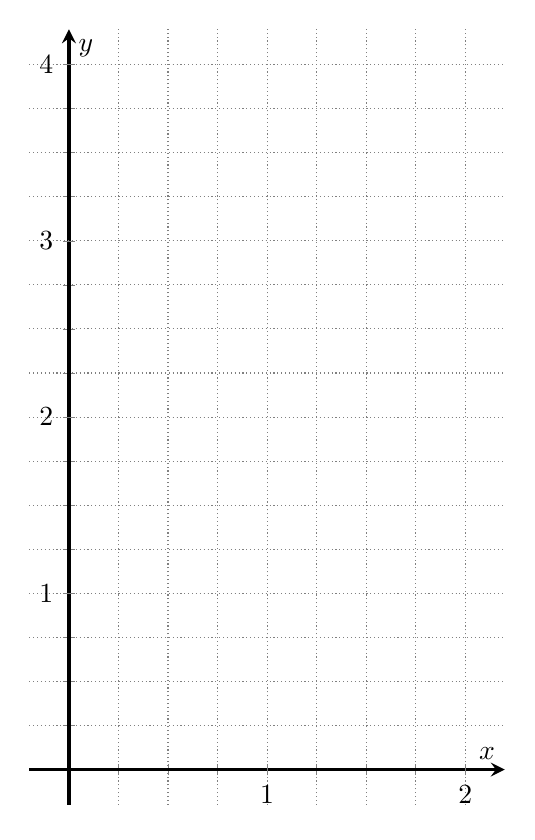
\begin{tikzpicture}[baseline=(current bounding box.north)]
	\begin{axis}[
			width=3in,height=4.5in,
			xticklabels={},
			yticklabels={},
			extra x ticks={1,2},
			extra y ticks={1,2,3,4},
			axis lines=middle,
			axis line style={very thick},
			grid style={thin,densely dotted,black!50},
			grid=major,
			xtick distance=.25, ytick distance=.25,
			xmin=-0-.2, xmax=2+.2,
			ymin=-0-.2, ymax=4+.2,
			xlabel=$x$,
			ylabel=$y$]
	\end{axis}
\end{tikzpicture}
\\[1em]
In your own words, how does the vertical stretch affect the graph?
\\[5em]
Given a parabola, how could you determine the vertical stretch of its equation?
\clearpage
The formula for a quadratic function is:
\[
	y=a(x-h)^2+k
\]
where $a$ represents the vertical stretch, and $(h,k)$ is the vertex of the parabola.
\subsubsection*{Negative $a$}
What happens when $a$ is negative?  Try graphing $y=-1(x+1)^2-1$.  We know where the vertex is.  Which direction does the parabola open?\\
\blankgraph{-4}{4}{-8}{8}{3}{6}

When working with a quadratic function, there are several properties we need to take note of:
\begin{itemize}
	\item vertex: $(h,k)$
	\item axis of symmetry: $x=h$
	\item vertical stretch: $a$
	\item direction of opening: sign of $a$
	\item $x$-intercepts, and how many exist
	\item $y$-intercept
\end{itemize}

\clearpage
\prb{Sketch each function.
	\begin{tasks}(2)
		\task $y=2(x+1)^2-3$\\
		\blankgraph{-4}{2}{-4}{2}{3}{3}
		\task $y=-1(x-3)^2+1$\\
		\blankgraph{-1}{5}{-4}{2}{3}{3}
		\task $y=\frac{1}{2}(x-1)^2-1$\\
		\blankgraph{-2}{4}{-2}{4}{3}{3}
		\task $y=-\frac{1}{2}x^2-3$\\
		\blankgraph{-3}{3}{-5}{1}{3}{3}
	\end{tasks}
}
\sol{
	\begin{tasks}(2)
		\task
		\curve{2*(x+1)^2-3}{-4}{2}{-4}{2}{}{<->}
		\task
		\curve{-1*(x-3)^2+1}{-1}{5}{-4}{2}{}{<->}
		\task
		\curve{.5*(x-1)^2-1}{-2}{4}{-2}{4}{}{<->}
		\task
		\curve{-.5*x^2-3}{-3}{3}{-5}{1}{}{<->}
	\end{tasks}
}

\prb{Expand the expression $(2x+2)(x-2)$.  Is it quadratic?\\[3em]}
\sol{Yes, the expression $(2x+2)(x-2)=2x^2-2x-4$ is quadratic.}

\prb{Expand the expression $2(x-\frac 12)^2 - \frac 92$.  Does it look familiar?\\[3em]}
\clearpage
\prb{Graph the function $2(x-\frac 12)^2 - \frac 92$ (the expression from the above two questions).  State the $x$-intercepts.\\
	\blankgraph{-2}{4}{-5}{1}{3}{3}
}
\sol{
	\curve{2*x^2-2*x-4}{-2}{4}{-5}{1}{}{<->}
	\\
	The $x$-intercepts are $x=-1$ and $x=2$.
}

\prb{Is there anything about the expression $(2x+2)(x-2)$ that makes you think that the $x$-intercepts are $x=-1$ and $x=2$?}

\prb{Find the vertex and vertical stretch of each function to write it in vertex form, and then re-write each one in standard form.
	\begin{tasks}(2)
		\task
		\curve{2*(x-1)^2-2}{-2}{4}{-4}{2}{}{<->}
		\task
		\curve{-1*(x+1)^2+1}{-4}{2}{-5}{1}{}{<->}
		\task
		\curve{.5*(x+1)^2-2}{-4}{2}{-3}{3}{}{<->}
		\task
		\curve{-.5*x^2-1}{-3}{3}{-5}{1}{}{<->}
		\task
		\curve{.5*(x-1)^2+1}{-2}{4}{-2}{4}{}{<->}
		\task
		\curve{-3*(x-1)^2+5}{-2}{4}{-1}{5}{}{<->}
	\end{tasks}}
\sol{
	\begin{tasks}(2)
		\task $y= 2       (x-1)^2-2 =  2 x^2 - 4 x$
		\task $y=-1       (x+1)^2+1 = -x^2 - 2 x$
		\task $y=\frac 12 (x+1)^2-2 = \frac 12 x^2 + x - \frac 32$
		\task $y=-\frac 12(x-0)^2-1 = \frac 12x^2-1$
		\task $y=\frac 12 (x-1)^2+1 = \frac 12 x^2 - x + \frac 32$
		\task $y=-3       (x-1)^2+5 = -3 x^2 + 6 x + 2$
	\end{tasks}
}
\prb{Find the number of $x$-intercepts of each quadratic function, without graphing it.
	\begin{tasks}(2)
		\task $y=-2(x-1)^2+1$
		\task $y=-2(x-1)^2-1$
		\task $f(x)=-2(x-1)^2$
		\task $g(x)=2(x+1)^2+1$
		\task $P(x)=3x^2-1$
		\task $Q(x)=-3x^2-1$
	\end{tasks}
}
\sol{
	\begin{tasks}(6)
		\task 2
		\task 0
		\task 1
		\task 0
		\task 1
		\task 0
	\end{tasks}
}

\chapter{4. Completing the Square}
Sometimes a quadratic function isn't given to us in vertex form.  This makes graphing it difficult.  Luckily it's not very difficult to convert from ``general form'' to vertex form.
\\[1em]
We say that a quadratic function is in general form when it looks something like this:
\[
	y=ax^2+bx+c
\]
where $a,b,$ and $c$ are real numbers, and $a\ne 0$.  If $a=0$ then the function is no longer quadratic, it's linear.  An example of a quadratic in general form is $y=2x^2+x-1$.
\\[1em]
To convert a general-form-quadratic into vertex form, we first must be able to recognize perfect squares.  This is because a quadratic function in vertex form \emph{begins} with a perfect square: $y=a(x-h)^2+k$.  The $(x-h)^2$ is the perfect square.
\\[1em]
One type of perfect square is a linear function that has been squared.  Try expanding these perfect squares:
\begin{tasks}(2)
	\task $(x+1)^2$\\[3em]
	\task $(x-1)^2$\\[3em]
	\task $(x+3)^2$\\[3em]
	\task $(x-3)^2$\\[3em]
	\task $(2x-1)^2$\\[3em]
	\task $(2x+1)^2$\\[3em]
	\task $(-3x+1)^2$\\[3em]
	\task $(-3x-1)^2$\\[3em]
\end{tasks}
What do you notice?  How can you recognize a perfect square that has been expanded?
\\[2em]
Is $x^2+3x+1$ a perfect square?  How can you tell?
\\[2em]
Is $x^2+8x+16$ a perfect square?  How can you tell?
\clearpage
Suppose the following general-form-quadratics were perfect squares. Fill in the blank.\\[1em]
\begin{tasks}(2)
	\task $x^2+2x+\underline{\hspace{3em}}$\\[2em]
	\task $x^2-2x+\underline{\hspace{3em}}$\\[2em]
	\task $x^2+6x+\underline{\hspace{3em}}$\\[2em]
	\task $x^2-6x+\underline{\hspace{3em}}$\\[2em]
	\task $x^2+8x+\underline{\hspace{3em}}$\\[2em]
	\task $x^2-10x+\underline{\hspace{3em}}$\\[2em]
	\task $x^2-5x+\underline{\hspace{3em}}$\\[2em]
	\task $x^2+9x+\underline{\hspace{3em}}$\\[2em]
\end{tasks}
The process of filling in the blank like we just did is called ``completing the square'' when we are done we are left with a perfect square.
\\[1em]
Considers doing the same process using the area model for multiplication.  Complete the above problems using the area model.
\clearpage
\
\clearpage
We can use the process of completing the square to convert a quadratic equation in general form into a quadratic in vertex form.  This allows us to graph them very easily.
\\[1em]
Use the process of completing the square to write the quadratic function in vertex form. Then graph the function.
\[y=x^2-2x+3\]
\blankgraph{-2}{8}{-1}{9}{4}{4}
\vfill
Use the process of completing the square to write the quadratic function in vertex form. Then graph the function.
\[y=2x^2+6x+3\]
\blankgraph{-6}{4}{-5}{5}{4}{4}
\vfill
\clearpage
\prb{Write the formula for a quadratic function in vertex form.}
\sol{$y=a(x-h)^2+k$}
\prb{Convert each equation from standard form into vertex form.  State the vertex and vertical stretch.  Verify your answers by graphing them in Desmos.
	\begin{tasks}(2)
		\task $y=2 x^2-12 x$\\[10em]
		\\Vertex:
		\\Vertical Stretch:
		\task $y=6 x^2+24 x+17$\\[10em]
		\\Vertex:
		\\Vertical Stretch:
		\task $y=10 x^2-160 x+80$\\[10em]
		\\Vertex:
		\\Vertical Stretch:
		\task $y=3 x^2+42 x-96$\\[10em]
		\\Vertex:
		\\Vertical Stretch:
		\task $f(x)=-4 x^2+16 x$\\[10em]
		\\Vertex:
		\\Vertical Stretch:
		\task $g(x)=-20 x^2-400 x-243$\\[10em]
		\\Vertex:
		\\Vertical Stretch:
		\task $h(x)=-x^2-42 x+500$\\[10em]
		\\Vertex:
		\\Vertical Stretch:
		\task $k(x)=-7 x^2+182 x-70$\\[10em]
		\\Vertex:
		\\Vertical Stretch:
		\task $y=x^2+\frac{3}{2} x-7$\\[10em]
		\\Vertex:
		\\Vertical Stretch:
		\task $y=-x^2-\frac{3}{8} x$\\[10em]
		\\Vertex:
		\\Vertical Stretch:
		\task $y=2 x^2-\frac{5}{6} x+1$\\[10em]
		\\Vertex:
		\\Vertical Stretch:
		\task $y=-2 x^2+8 x-3$\\[10em]
		\\Vertex:
		\\Vertical Stretch:
	\end{tasks}
}

\prb{Determine the minimum or maximum value of each quadratic function.  \\ Hint: convert decimals into reduced fractions to save a headache!
	\begin{tasks}(2)
		\task $f(x)=x^2+5 x+3$
		\\[10em]
		\task $f(x)=2 x^2-2 x+1$
		\\[10em]
		\task $f(x)=-0.5 x^2+10 x-3$
		\\[10em]
		\task $f(x)=3 x^2-4.8 x$
		\\[10em]
		\task $f(x)=-0.2 x^2+3.4 x+4.5$
		\\[10em]
		\task $f(x)=-2 x^2+5.8 x-3$
		\\[10em]
	\end{tasks}
}

\prb{Solve each equation.  Remember: if $x^2=a$ then $x=\pm \sqrt a$.  For some questions, you may need to complete the square.
	\begin{tasks}(2)
		\task $x=1, x=5$
		\\[5em]
		\task $x=-5, x=1$
		\\[5em]
		\task $d=-\frac{3}{2}, d=\frac{1}{2}$
		\\[5em]
		\task $h=\frac{3 \pm \sqrt{7}}{4}$
		\\[5em]
		\task $s=\frac{-12 \pm \sqrt{3}}{2}$
		\\[5em]
		\task $x=-4 \pm 3 \sqrt{2}$
		\\[5em]
		\task $(x-3)^2=4$
		\\[5em]
		\task $(x+2)^2=9$
		\\[5em]
		\task $\left(d+\frac{1}{2}\right)^2=1$
		\\[5em]
		\task $\left(h-\frac{3}{4}\right)^2=\frac{7}{16}$
		\\[5em]
		\task $(s+6)^2=\frac{3}{4}$
		\\[5em]
	\end{tasks}
}
\sol{
	\begin{tasks}(2)
		\task $x=1, x=5$
		\task $x=-5, x=1$
		\task $d=-\frac{3}{2}, d=\frac{1}{2}$
		\task $h=\frac{3 \pm \sqrt{7}}{4}$
		\task $s=\frac{-12 \pm \sqrt{3}}{2}$
		\task $x=-4 \pm 3 \sqrt{2}$
		\task $x=-5 \pm \sqrt{21}$
		\task $x=4 \pm \sqrt{3}$
		\task $x=-1 \pm \sqrt{\frac{2}{3}}$
		\task $x=1 \pm \sqrt{\frac{5}{2}}$
		\task $x=-3 \pm \sqrt{13}$
		\task $x=4 \pm 2 \sqrt{7}$
	\end{tasks}
}

\prb{The managers of a business are examining
	costs. It is more cost-effective for them
	to produce more items. However, if too
	many items are produced, their costs
	will rise because of factors such as
	storage and overstock. Suppose that
	they model the cost, C, of producing
	n thousand items with the function
	C(n) = 75n2 - 1800n + 60 000.
	Determine the number of items
	produced that will minimize their costs.\\[2in]}
\sol{12000 items.}

\prb{A gymnast is jumping on a trampoline.
	His height, $h$, in metres, above the floor
	on each jump is roughly approximated
	by the function $h(t) = -5t2 + 10t + 4$,
	where $t$ represents the time, in seconds,
	since he left the trampoline. Determine
	algebraically his maximum height on
	each jump.\\[2in]}
\sol{9 m}

\prb{A concert promoter is planning the ticket
	price for an upcoming concert for a certain
	band. At the last concert, she charged
	\$70 per ticket and sold 2000 tickets. After
	conducting a survey, the promoter has
	determined that for every \$1 decrease
	in ticket price, she might expect to sell
	50 more tickets.
	\begin{tasks}
		\task What maximum revenue can the
		promoter expect? What ticket price
		will give that revenue?\\[1in]
		\task How many tickets can the promoter
		expect to sell at that price?\\[1in]
		\task Explain any assumptions the concert
		promoter is making in using this
		quadratic function to predict revenues.\\[1in]
	\end{tasks}
}
\sol{
	\begin{tasks}
		\task The maximum revenue is \$151 250 when the ticket price is \$55.
		\task 2750 tickets
		\task Example: Assume that the decrease in ticket prices determines the same increase in ticket sales as indicated by the survey.
	\end{tasks}
}

\prb{A rectangle has length $5x+15$ and width $31-2x$.  What is the value of $x$ that gives the largest area?}
\sol{$\frac{25}{4}$}










\chapter{5. Factoring}
A perfect square has at least two factors.  The factors of $x^2$ are $x$ and $x$.  Some people say that $x$ is a factor of $x^2$ with \emph{multiplicity} two, because it is a factor two times.
\\[1em]
Factoring a quadratic equation can be done in several ways, but one of the more efficient ways is to notice what happens when we multiply two linear functions:
\[
    (x+a)(x+b) =
\]
What is the relationship between $a$, $b$, and the quadratic?  Could you go backwards?
\\[1in]
What about a ``larger'' product of linear functions?  In other words, what if we have coefficients on $x$?
\[ 
    (ax+b)(cx+d) = 
\]
How can you use the ``diamond method'' to factor this?
\\[2in]
\subsection*{Special Factors}
Some quadratics have a specific pattern.  Consider the following two products:
\[
    (a+b)(a-b) = 
    \hfill 
    (a+b)(a+b) =
    \hfill 
\]
The first is called a difference of squares, and the second is called a perfect square.  Why do you think they're called this?
\vfill 
\clearpage
Factor all of the below quadratics.
\begin{tasks}(2)
	\task $x^2+11x + 30$\\[2em]
	\task $5x^2 - 20 $\\[2em]
	\task $x^2-10x +21 $\\[2em]
	\task $4x^2 + 24x $\\[2em]
	\task $20x^2+88x-192 $\\[2em]
	\task $2x^2 -11x -40 $\\[2em]
	\task $10x^2 -24x -18 $\\[2em]
	\task $12x^2-4x-8$\\[2em]
\end{tasks}
\section*{Don't forget to remove common factors.}
Some quadratics have common factors in all of their terms.  It is very useful to factor that out first.  Try it on the following quadratics.
\begin{tasks}(3)
\task $5 x+10$
\task $3 x^2-6$
\task $12 x^4-8 x^3+4 x^2$
\end{tasks}
\vspace{1.5in}
\section*{What does factoring have to do with graphing?}
There is a very important property in algebra called the zero factor theorem.  It says that for any two numbers $a$ and $b$, if $a\times b = 0$ then either $a=0$ or $b=0$; note that this is not an exclusive ``or,'' so another possibility is that $a=b=0$. 

This can help us find the $x$-intercepts of a quadratic.  To find an $x$-intercept, we set $y=0$ and solve for $x$.
\\[1em]
Find the $x$-intercepts of the following quadratic:
\[y=x^2-5x-24\]
\vfill How do you find the $y$-intercept?
\clearpage
\section*{What about quadratics that don't have roots?}
The quadratic function $y=x^2+1$ does not pass through the $x$-axis and does not have any roots.  Can you factor this quadratic?  Try it!
\\[4em]
What about $y=x^2 - 2$?  This function definitely has two roots since it opens upwards but has a vertex below the $x$ axis.  Using algebra, we can set $y=0$ and solve for $x$ to get $x=\pm \sqrt 2$.  Try expanding $(x+\sqrt 2)(x-\sqrt 2)$.  Notice anything?
\\[4em]
Some quadratics have no roots and they're impossible to factor for that reason.  Some quadratics do have roots but are nearly impossible to factor.  That's because their roots are irrational, and include a square root.  All of the quadratics in the exercises of this chapter will have rational roots.  In the next chapter we'll figure out how to find the roots of any quadratic - even those that have irrational roots.

\prb {Multiply.
    \begin{tasks}
\task $(2 x+1)(3 x+2)$
		\\[5em]
\task $(3 y-4)(2 y+3)$
		\\[5em]
\task $\left(3 x^2+4\right)(x+1)$
		\\[5em]
\task $\left(4 y^2+3\right)(3 y-1)$
		\\[5em]
\task $(-3 y-4)(2 y-3)$
		\\[5em]
\task $(5 x-y)(5 x-y)$
		\\[5em]
\task $(2 x-1)\left(2 x^2+3 x-1\right)$
		\\[5em]
\task $(5 x-6)\left(2 x^2+7 x-3\right)$
		\\[5em]
\task $(3 y-2 x)\left(4 y^2-3 x y+x^2\right)$
		\\[5em]
\task $\left(x^2+2 y\right)\left(2 x^2+3 x y-y^2\right)$
		\\[5em]
\task $(4-x)\left(4-3 x^3+x^2-5 x\right)$
		\\[5em]
\task $(2-y)\left(3-2 y^2-y^3+4 y\right)$
		\\[5em]
\task $(x-y)\left(x^2+x y+y^2\right)$
		\\[5em]
\task $\left(x^2-y^2\right)\left(x^4+x^2 y^2+y^4\right)$
		\\[5em]
\task $\left(3 x^2-x+5\right)\left(2 x^2+4 x-1\right)$
		\\[5em]
\task $\left(2 y^2+y-7\right)\left(5 y^2-3 y-1\right)$
		\\[5em]
\end{tasks}
}
\sol{
    \begin{tasks}(2)
\task $6 x^2+7 x+2$
\task $6 y^2+y-12$
\task $3 x^3+3 x^2+4 x+4$
\task $12 y^3-4 y^2+9 y-3$
\task $-6 y^2+y+12$
\task $25 x^2-10 x y+y^2$
\task $4 x^3+4 x^2-5 x+1$
\task $10 x^3+23 x^2-57 x+18$
\task $12 y^3-17 x y^2+9 x^2 y-2 x^3$
\task $2 x^4+3 x^3 y-x^2 y^2+4 x^2 y+6 x y^2-2 y^3$
\task $3 x^4-13 x^3+9 x^2-24 x+16$
\task $y^4-8 y^2+5 y+6$
\task $x^3-y^3$
\task $x^6-y^6$
\task $6 x^4+10 x^3+3 x^2+21 x-5$
\task $10 y^4-y^3-40 y^2+20 y+7$
\end{tasks}
}
\prb{Factor completely.
	\begin{tasks}(2)
		\task $x^2+7 x+10$
		\\[5em]
		\task $5 z^2+40 z+60$
		\\[5em]
		\task $0.2 d^2-2.2 d+5.6$
		\\[5em]
		\task $3 y^2+4 y-7$
		\\[5em]
		\task $8 k^2-6 k-5$
		\\[5em]
		\task $0.4 m^2+0.6 m-1.8$
		\\[5em]
		\task $x^2+x-20$
		\\[5em]
		\task $x^2-12 x+36$
		\\[5em]
		\task $\frac{1}{4} x^2+2 x+3$
		\\[5em]
		\task $2 x^2+12 x+18$
		\\[5em]
		\task $4 y^2-9 x^2$
		\\[5em]
		\task $0.36 p^2-0.49 q^2$
		\\[5em]
		\task $\frac{1}{4} s^2-\frac{9}{25} t^2$
		\\[5em]
		\task $0.16 t^2-16 s^2$
		\\[5em]
		\task $(x+2)^2-(x+2)-42$
		\\[5em]
		\task $6\left(x^2-4 x+4\right)^2+\left(x^2-4 x+4\right)-1$
		\\[5em]
		\task $(4 j-2)^2-(2+4 j)^2$
		\\[5em]
	\end{tasks}
}
\sol{
	\begin{tasks}(2)
		\task $(x+2)(x+5)$
		\task $5(z+2)(z+6)$
		\task $0.2(d-4)(d-7)$
		\task $(y-1)(3 y+7)$
		\task $(4 k-5)(2 k+1)$
		\task $0.2(2 m-3)(m+3)$
		\task $(x+5)(x-4)$
		\task $(x-6)^2$
		\task $\frac{1}{4}(x+2)(x+6)$
		\task $2(x+3)^2$
		\task $(2 y+3 x)(2 y-3 x)$
		\task $(0.6 p+0.7 q)(0.6 p-0.7 q)$
		\task $\left(\frac{1}{2} s+\frac{3}{5} t\right)\left(\frac{1}{2} s-\frac{3}{5} t\right)$
		\task $(0.4 t+4 s)(0.4 t-4 s)$
		\task $(x+8)(x-5)$
		\task $\left(2 x^2-8 x+9\right)\left(3 x^2-12 x+11\right)$
		\task $(-4)(8 j)$
	\end{tasks}
}

\prb{If a quadratic function has one root at $x=4$ and another root at $x=6$, where is the axis of symmetry?\\[5em]}
\sol{The axis of symmetry will always be exactly in the middle of the two roots.  Taking the average of the two roots gives $\frac{4+6}{2}=5$.}

\prb{The roots of the quadratic function $y=x^2-4x-12$ are $6$ and $-2$.  Without completing the square, determine the vertex.\\[5em]}
\sol{The axis of symmetry will be the average of the roots, or $x=1$.  When $x=1$ $y=-15$.  So the vertex is found at $(1,-15)$.}

\prb{Solve each equation by setting one side equal to zero and factoring.
	\begin{tasks}(2)
		\task $k^2-5 k=0$
		\\[5em]
		\task $9 x^2=x+8$
		\\[5em]
		\task $\frac{8}{3} t+5=-\frac{1}{3} t^2$
		\\[5em]
		\task $\frac{25}{49} y^2-9=0$
		\\[5em]
		\task $2 s^2-4 s=70$
		\\[5em]
		\task $4 q^2-28 q=-49$
		\\[5em]
	\end{tasks}
}
\sol{
	\begin{tasks}(3)
		\task 0 and 5
		\task $-\frac{8}{9}$ and 1
		\task $-5$ and $-3$
		\task $-\frac{21}{5}$ and $\frac{21}{5}$
		\task $-5$ and 7
		\task $\frac{7}{2}$
	\end{tasks}
}
\prb{A square has an area of $\left(9 x^2+30 x y+25 y^2\right)$ square centimetres. What is an expression for the perimeter of the square?\\[5em]}
\sol{$4(3x + 5y)$ centimetres.}
\prb{Determine the shaded area in factored form, if the circles are each of radius $r$.
    \\
  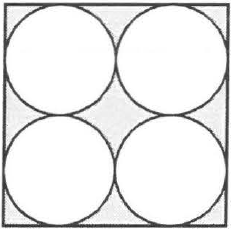
\includegraphics[height=2in]{figures/circlesinsquare.png}
}
\prb{Determine the shaded area of the equilateral triangle in factored form.
\\
  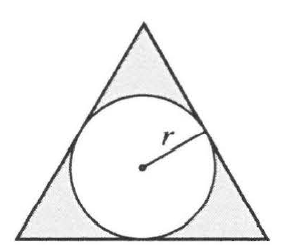
\includegraphics[height=2in]{figures/circleintriangle.png}
}
\prb{Determine the shaded area in factored form.
\\
  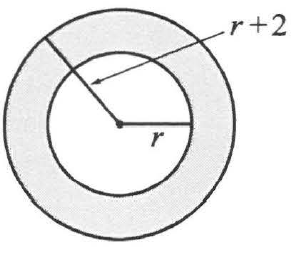
\includegraphics[height=2in\textwidth]{figures/circle-in-circle.png}
}
\prb{Ellie factored $4-12 y+9 y^2$ as $(3 y-2)^2$, while Kate factored it as $(2-3 y)^2$. Who was correct? Why?}
\chapter{6. The Quadratic Formula}
Some quadratics are hard to factor.  Some quadratics can't be factored at all.  This raises an important question: when you're having a hard time factoring a quadratic, how do you know if it's just hard, or that it's impossible? 
\\[1em]
The following two functions cannot be factored using the methods we know about.  Try completing the square and then graphing them.
\begin{tasks}(2)
	\task $y=x^{2}+2x-4$\\[4em]
	\blankgraph{-6}{4}{-6}{4}{3}{3}
	\task $y=x^{2}+2x+2$\\[4em]
	\blankgraph{-6}{4}{-2}{8}{3}{3}
\end{tasks}
Since neither of these can be factored, without graphing them, how can we tell which one has roots and which one doesn't?
\\[1em]
In function a) set $y=0$ and isolate $x$ by moving the constant to the other side of the equation and then taking the square root of both sides.
\\[1em]
Before you do that, remember that even though $x^2=1$ means that $x=1$ or $x=-1$, it is not true that $\sqrt 1 = \pm 1$.  When we take the square root of a number, we get the \emph{principle} square root, which is always positive.  When we solve an equation that has a square in it, since we need to account for the fact that the base of the power is negative, we include the $\pm$ in our solution.
\clearpage
Do the same process for function b).
\\[3in]
To save time, mathematicians devised a formula that allows us to skip the process of completing the square, and to get the roots of a quadratic function directly.  This method will also tell us immediately if a quadratic function has no roots.
\\[1em]
The quadratic formula can be derived from a gerneral quadratic $y=ax^2+bx+c$.
\clearpage
\section*{The Quadratic Formula}
If $ax^2+bx+c=0$ then ${\displaystyle x=\frac{-b\pm \sqrt{b^2-4ac}}{2a}}$.
\\[1em]
Use the quadratic formula to find the roots of the following functions.
\begin{tasks}(2)
	\task$y = x^2 + 4x - 12$\\[2.5in]
	\task$y = 5x^2 -18 x + 9$\\[2.5in]
	\task$y = 2x^2 -21x + 40$\\[2.5in]
	\task$y = 35x^2 + 71x +24 $\\[2.5in]
	\task$y = 4x^2 + 7x $\\[2.5in]
	\task$y = x^2 - 9 $\\[2.5in]
\end{tasks}
Remember that not all quadratic functions have roots.  How does the quadratic formula handle this?
\section*{The Discriminant}
Every square root (and $n$-th root) has what's called a ``radicand.''  This is the portion underneath the root symbol.  In $\sqrt9$ the radicand is 9.
\\[1em]
When taking a square root, if our radicand is negative, our square root is not a real number.  In other words, we can write
\[\sqrt{-1}\not\in\mathbb R.\]
Keep in mind that $\sqrt{-1}$ \emph{is} defined, it's just not a real number.
\\[1em]
The radicand in the quadratic formula is called the discriminant.  It is because it is able to discriminate between quadratic functions that have 2 roots, 1 root, and no roots.
\\[1em]
Let $D$ be the discriminant.  In other words, $D=b^2-4ac$.  When this is the case we can write the quadratic formula in the following way:
\[x=\frac{-b\pm \sqrt{D}}{2a}\]
which leads us to three possibilities about $D$.
\begin{enumerate}
	\item If $D>0$ then $\pm \sqrt{D}$ has two values: $\sqrt D$ and $-\sqrt D$.
	\item If $D=0$ then $\pm \sqrt{D}=\pm 0 = 0$ which is just one value.
	\item If $D<0$ then $\pm \sqrt{D}$ is undefined because $\sqrt{D}$ is undefined.
\end{enumerate}
In your own words, write what impact the discriminant has on the number of roots on a quadratic function.

\prb{Use the discriminant to determine the
	number of solutions to each equation.  Check your answers by graphing the function with Desmos.
	\begin{tasks}(2)
		\task $x^2-7 x+4=0$ \\[3em]
		\task $s^2+3 s-2=0$ \\[3em]
		\task $r^2+9 r+6=0$ \\[3em]
		\task $n^2-2 n+1=0$ \\[3em]
		\task $7 y^2+3 y+2=0$ \\[3em]
		\task $4 t^2+12 t+9=0$ \\[3em]
	\end{tasks}
}

\sol{
	\begin{tasks}(3)
		\task 2
		\task 2
		\task 2
		\task 1
		\task 0
		\task 1
	\end{tasks}
}
\clearpage
\prb{Use the quadratic formula to solve each
	quadratic equation.  Make sure one side is equal to zero.
	\begin{tasks}(2)
		\task $7 x^2+24 x+9=0$\\[5em]
		\task $4 p^2-12 p-9=0$\\[5em]
		\task $3 q^2+5 q=1$\\[5em]
		\task $2 m^2+4 m-7=0$\\[5em]
		\task $2 j^2-7 j=-4$\\[5em]
		\task $16 g^2+24 g=-9$\\[5em]
	\end{tasks}
}

\sol{
	\begin{tasks}(3)
		\task $x=-3, x=-\frac{3}{7}$
		\task $p=\frac{3 \pm 3 \sqrt{2}}{2}$
		\task $q=\frac{-5 \pm \sqrt{37}}{6}$
		\task $m=\frac{-2 \pm 3 \sqrt{2}}{2}$
		\task $j=\frac{7 \pm \sqrt{17}}{4}$
		\task $g=-\frac{3}{4}$
	\end{tasks}
}

\prb{How many methods have we learned to solve a quadratic equation?\\[4em]}
\sol{Five methods: The Quadratic Formula, completing the square and isolating $x$, factoring, taking the square root, and graphing.}

\prb{Solve the equation using the best method.  State the method.
	\begin{tasks}(2)
		\task $n^2+2 n-2=0$
		\\[8em]
		\task $-y^2+6 y-9=0$
		\\[8em]
		\task $-2 u^2+16=0$
		\\[8em]
		\task $\frac{x^2}{2}-\frac{x}{3}=1$
		\\[8em]
		\task $x^2-4 x+8=0$
		\\[8em]
	\end{tasks}
}
\sol{
	\begin{tasks}(2)
		\task $n=-1 \pm \sqrt{3}$; complete the square
		\task $y=3$; factor
		\task $u=\pm 2 \sqrt{2}$; square root
		\task $x=\frac{1 \pm \sqrt{19}}{3} ;$ quadratic formula
		\task no real roots; graphing
	\end{tasks}
}

\prb{An open-topped box is being made from
	a piece of cardboard measuring 12 in. by
	30 in. The sides of the box are formed
	when four congruent squares are cut from
	the corners, as shown in the diagram. The
	base of the box has an area of 208 sq. in..
	\begin{tasks}
		\task Create a diagram.
		\\[10em]
		\task What equation represents the surface area of the base of the box?
		\\[4em]
		\task What is the side length, $x$, of the square cut from each corner?
		\\[4em]
		\task What are the dimensions of the box?
		\\[4em]
	\end{tasks}
}
\sol{
	\begin{tasks}
		\task Make your own diagram!
		\task $(30-2 x)(12-2 x)=208$.
		\task $2 \mathrm{in}$.
		\task 8 in. by 26 in. by 2 in.
	\end{tasks}
}

\prb{Two small private planes take off from the same airport. One plane flies north at $150 \mathrm{~km} / \mathrm{h}$. Two hours later, the second plane flies west at $200 \mathrm{~km} / \mathrm{h}$. How long after the first plane takes off will the two planes be $600 \mathrm{~km}$ apart? Use Desmos to express your answer to the nearest tenth of an hour.}
\sol{3.5 hours.}













\chapter{7. Complex Numbers}
When we come across a quadratic expression that has a negative discriminant, we say that there are no real roots.  Does that mean that there actually are roots, but they're just not real?  What does it mean for a number to not be real?  It means it must be imaginary!
\\[1em]
To understand how we can use a number that is not real, it may help to look back into history to see how humans had to work very hard to accept numbers that we find simple today.
\\[1em]
Humans have seemingly always known about proportional numbers like fractions.  In fact our friend Pythagoras (who named the Pythagorean Theorem after himself, despite it being a popular theorem around the globe for several hundred years before him) believed that every number was the ratio of two whole numbers.  When his friend Hippasus proved that some numbers are not rational, Pythagoras killed him!
\\[1em]
All the while, no human had ever used the number zero.  After all, why would somebody use a number, which represents quantity, to describe something that has no quantity?  Sometimes humans would use a number like zero to record large numbers like 100 or 1000.  But the first account of humans writing down a value for 0 wasn't until around the year 3 BCE.  Keep in mind that this is several thousand years \emph{after} humans first proved the Pythagorean Theorem.
\\[1em]
It wasnt until about two hundred years after humans accepted 0 into their arithmatic that we allowed negative numbers into the mix.  Before then, the answer to the question $x+5=3$ was ``no solution.''
\\[1em]
In 1872 a mathematician called Richard Dedekind formally defined the set of real numbers.  He did this by taking the set of rational numbers and ``cutting'' them in a clever way, using what was later called ``Dedekind cuts.''
\\[1em]
Believe it or not, but before Dedekind was born humans were using imaginary numbers.  So before real numbers were properly defined, we were able to take the square root of a negative number.
\\[3em]
Taking the square root of a negative number is easy.  All you need to know is this:
\begin{enumerate}
	\item $\sqrt{ab}=\sqrt a \sqrt b$
	\item $\sqrt{-1}=i$
\end{enumerate}
The number $i$ is called the imaginary unit and its definition is that it is the principle square root of $-1$.
\\[1em]
Calculate the following:
\begin{tasks}(3)
	\task $\sqrt{-9}$
	\task $\sqrt{-20}$
	\task $5\sqrt{-300}$
\end{tasks}
\clearpage
With the knowledge of imaginary numbers, can you calculate the roots of the function $y=-2x^{2}+3x-4$?
\\[4em]
When a quadratic has roots that are not real, we call that quadratic an ``irriducible quadratic'' because you cannot reduce it, i.e. you cannot factor it.
\subsubsection*{Complex Numbers}
A complex number is a number that has a real part and an imaginary part, like $1+i$ or $3-\sqrt2 i$.  The real part is the first number and the imaginary part is the multiple of $i$.  \\[1em]
Adding complex numbers is easy: just add the real part and add the imaginary part.  Try the following:
\begin{tasks}(3)
	\task $\left(2+3i\right) + \left(3-5i\right)$\\[2em]
	\task $\left(\frac 12-3i\right) + \left(3-\frac 34i\right)$\\[2em]
	\task $\left(\sqrt 2+3i\right) + \left(\sqrt 2-5i\right)$\\[2em]
\end{tasks}
\subsubsection*{Complex Conjugates}
The conjugate of the complex number $a+bi$ is $a-bi$.  This can come in handy when dividing complex numbers.  When evaluating a quotient of complex numbers, we multiply the numerator and denominator by the conjugate of the denominator.  This will always cancel out the $i$ in the denominator.
\\[1em]
Try doing that with $\displaystyle \frac{2+i}{3-2i}$.
\\[4em]
\subsubsection*{Special Cases}
When working with complex numbers, all of our laws of algebra stay the same, but we have to be careful of one special rule.
\\[1em]
While it's true that $\sqrt{a}\sqrt{b}=\sqrt{ab}$ for \emph{positive} real numbers $a$ and $b$, it is not true that $\sqrt{-a}\sqrt{-b}=\sqrt{(-a)(-b)}$.  Try completing each equality below.
\begin{tasks}(2)
	\task $\sqrt{-1}\sqrt{-1} = \sqrt{(-1)(-1)}$
	\task $\sqrt{-1}\sqrt{-1} = i\cdot i$\\[4em]
\end{tasks}
This gives us a new rule:
\[
	\sqrt{-1}\sqrt{-1}\ne \sqrt{(-1)(-1)} = 1
\]
so when you are multiplying two roots of negatives, factor out an $i$ first.  So
\[
	\sqrt{-1}\sqrt{-1}=i\cdot i = -1.
\]
Try calculating $\sqrt{-12}\sqrt{-75}$ using the above rule.  Note that $\sqrt{-a}=i\sqrt{a}$.\\[4em]

\prb{Evaluate each radical expression.  Your answer should be in the form $a+bi$.
	\begin{tasks}(2)
		\task $\sqrt{-49}$ \\[4em]
		\task $\sqrt{-3} \sqrt{-12}$ \\[4em]
		\task $(3-\sqrt{-5})(1+\sqrt{-1})$ \\[4em]
		\task $\frac{2+\sqrt{-8}}{1+\sqrt{-2}}$ \\[4em]
	\end{tasks}
}

\sol{
	\begin{tasks}(4)
		\task $7 i \quad$
		\task $-6$
		\task $(3+\sqrt{5})+(3-\sqrt{5}) i$
		\task $2$
	\end{tasks}
}


\prb{Add or subtract.
	\begin{tasks}(2)
		\task $(3+2 i)+5 i$ \\[4em]
		\task $(5-3 i)+(-4-7 i)$ \\[4em]
		\task $(-6+6 i)+(9-i)$ \\[4em]
		\task $\left(7-\frac{1}{2}i\right)-\left(5+\frac{3}{2} i\right)$ \\[4em]
		\task $(-12+8 i)-(7+4 i)$ \\[4em]
	\end{tasks}
}

\sol{
	\begin{tasks}(5)
		\task $3+7 i$
		\task $1-10 i$
		\task $3+5 i$
		\task $2-2 i $
		\task $-19+4 i $
	\end{tasks}
}


\prb{Find each product, and write in the form $a+bi$.
	\begin{tasks}(2)
		\task $4(-1+2 i)$ \\[4em]
		\task $(7-i)(4+2 i)$ \\[4em]
		\task $(6+5 i)(2-3 i)$ \\[4em]
		\task $(2+5 i)(2-5 i)$ \\[4em]
		\task $(2+5 i)^2$ \\[4em]
	\end{tasks}
}

\sol{
	\begin{tasks}(5)
		\task $-4+8 i $
		\task $30+10 i$
		\task $27-8 i $
		\task $29 $
		\task $-21+20 i $
	\end{tasks}
}


\prb{Write each quotient, and express in the form $a+bi$.
	\begin{tasks}(2)
		\task $\displaystyle \frac{1}{i}$ \\[5em]
		\task $\displaystyle \frac{2-3 i}{1-2 i}$ \\[5em]
		\task $\displaystyle \frac{10 i}{1-2 i}$ \\[5em]
		\task $\displaystyle \frac{4+6 i}{3 i}$ \\[5em]
		\task $\displaystyle \frac{1}{1+i}-\frac{1}{1-i}$ \\[5em]
	\end{tasks}
}

\sol{
	\begin{tasks}(5)
		\task $-i $
		\task $\frac{8}{5}+\frac{1}{5} i$
		\task $-4+2 i$
		\task $2-\frac{4}{3} i$
		\task $-i$
	\end{tasks}
}




\prb{Find all solutions to the quadratic equation.
	\begin{tasks}(2)
		\task $x^2+49=0$ \\[8em]
		\task $x^2-x+2=0$ \\[8em]
		\task $x^2+3 x+7=0$ \\[8em]
		\task $x^2+x+1=0$ \\[8em]
		\task $2 x^2-2 x+1=0$ \\[8em]
		\task $6 x^2+12 x+7=0$ \\[8em]
	\end{tasks}
}

\sol{
	\begin{tasks}(3)
		\task $\displaystyle \pm 7 i$
		\task $\displaystyle \frac{1}{2} \pm \frac{\sqrt{7}}{2} i $
		\task $\displaystyle -\frac{3}{2} \pm \frac{\sqrt{19}}{2} i$
		\task $\displaystyle -\frac{1}{2} \pm \frac{\sqrt{3}}{2} i $
		\task $\displaystyle \frac{1}{2} \pm \frac{1}{2} i $
		\task $\displaystyle -1 \pm \frac{\sqrt{6}}{6} i$
	\end{tasks}
}












\chapter{8. Quadratic Equations}
A quadratic equation is an equation where at least one side of the equation is a quadratic expression, and the other side is either a constant, a linear expression, or another quadratic expression.  The following equations are quadratic equations.
\begin{enumerate}
	\item $x^2+2x-1=x^2+3x+2$
	\item $3=3x^2-8x$
	\item $2x^2-2x+4=3x-1$
\end{enumerate}
How many solutions could a quadratic equation have?  Why?\\[2in]
In order to solve a quadratic equation, we can follow the steps below:
\begin{enumerate}
	\item set one side of the equation equal to zero
	\item use the quadratic formula.
\end{enumerate}
Solve: $3x-2=5x^2-8x+2$
\clearpage
Quadratic equations can also be thought of as a system of non-linear equations, or a system of one non-linear equation and one linear equation.
\\[1em]
Use the axes below to show the number of ways two parabolas can intersect.\\[1em]
\blankaxes{2.3}{2}
\blankaxes{2.3}{2}
\blankaxes{2.3}{2}
\blankaxes{2.3}{2}
\\[1em]
Use the axes below to show the number of ways a parabola can intersect with a line.
\\[1em]
\blankaxes{2.3}{2}
\blankaxes{2.3}{2}
\blankaxes{2.3}{2}
\\[1em]
How many times does the function $y=2x-1$ intersect $y=3x^2-x-1$?  Is there a fast way of answering this?  Hint: can you make a single quadratic equation?  What is the discriminant?

\prb{State the number of solutions the quadratic system has, and then solve it.  Verify your answers in Desmos.
	\begin{tasks}(2)
		\task
		\begin{align*}
			y & =x^2     \\
			y & =2 x^2+x
		\end{align*}
		\task
		\begin{align*}
			y & =x^2   \\
			y & =2-x^2
		\end{align*}\\[8em]
		\task
		\begin{align*}
			y & =x^2       \\
			y & =3 x^2+8 x
		\end{align*}
		\task
		\begin{align*}
			y & =x^2+x       \\
			y & =2 x^2+3 x-3
		\end{align*}\\[8em]
		\task
		\begin{align*}
			y & =x^2-x       \\
			y & =2 x^2+2 x-4
		\end{align*}
		\task
		\begin{align*}
			y & =x^2+1     \\
			y & =2 x^2+x-3
		\end{align*}\\[8em]
		\task
		\begin{align*}
			y-x^2     & =0 \\
			x^2-2 x+y & =6
		\end{align*}
		\task
		\begin{align*}
			x^2+3 x-y-4 & =0 \\
			x^2+2 x+y-8 & =0
		\end{align*}\\[8em]
	\end{tasks}
}







\chapter{9. Tangents}
In Grade 9 we looked at a concept in circle geometry called tangents.  A tangent to a circle is a line that intersects a circle exactly once.  It turns out that tangents can exist in other contexts as well, but ``a line that intersects a parabola once'' is not necessarily a tangent.  Why do you think this is?
\\[1em]
\subsection*{Secant Lines}
Given any function $f(x)$, a secant line is a line that passes through two distinct points $(a,f(a))$ and $(b,f(b))$.  In other words, to create a secant line from a function, choose two points on that function and construct a line that passes through those two points.  That line is a secant line.
\\[1em]
Given the quadratic function below, we can choose any two points and construct the line that passes through thoses two points.  Remember: given two points, there is exactly one line that passes through both of those points.
\\[1em]
Which quadratic function is this?  And which line is the secant line?
\\
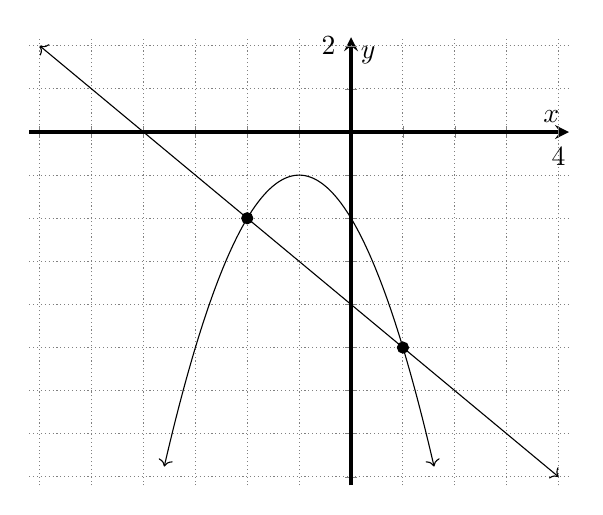
\begin{tikzpicture}[baseline=(current bounding box.north)]
	\begin{axis}[
			xticklabels={},
			yticklabels={},
			extra x ticks={4},
			extra y ticks={2},
			axis lines=middle,
			axis line style={very thick},
			grid style={thin,densely dotted,black!50},
			grid=major,
			xtick distance=1, ytick distance=1,
			xmin=-6-.2, xmax=4+.2,
			ymin=-8-.2, ymax=2+.2,
			xlabel=$x$,
			ylabel=$y$]
		\filldraw[black] (-2,-2) circle (2pt);
		\filldraw[black] (1,-5) circle (2pt);
		\addplot[
			domain=-3.6:1.6,
			samples=500,<->]
		(x,{-(x+1)^2-1});
		\addplot[
			domain=-6:4,
			samples=3,<->]
		(x,{-(x+2)-2});
	\end{axis}
\end{tikzpicture}
\\[1em]
On the quadratic function below, choose two points that are really close to each other and construct the line that passes through both points.
\\
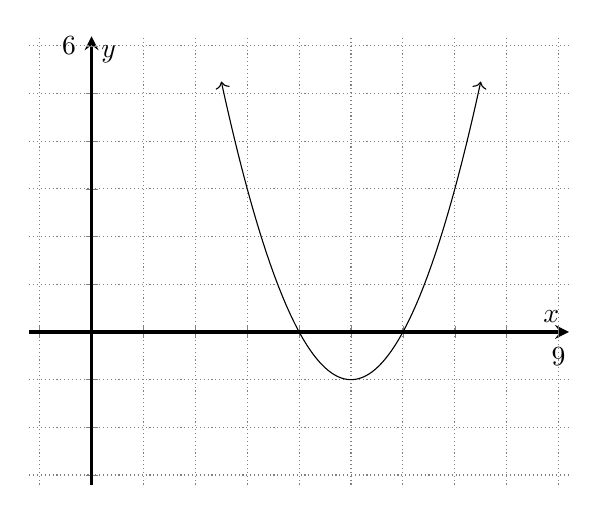
\begin{tikzpicture}[baseline=(current bounding box.north)]
	\begin{axis}[
			xticklabels={},
			yticklabels={},
			extra x ticks={9},
			extra y ticks={6},
			axis lines=middle,
			axis line style={very thick},
			grid style={thin,densely dotted,black!50},
			grid=major,
			xtick distance=1, ytick distance=1,
			xmin=-1-.2, xmax=9+.2,
			ymin=-3-.2, ymax=6+.2,
			xlabel=$x$,
			ylabel=$y$]
		\addplot[
			domain=2.5:7.5,
			samples=500,<->]
		(x,{(x-5)^2-1});
		\addplot[
			domain=0:5,
			samples=3,<->]
		(x,{-(x+2)-2});
	\end{axis}
\end{tikzpicture}
\subsection*{Secants to Tangents}
A tangent line can be constructed by making a secant line with two points that are infinitesmally close to each other.  To do this precisely, one should use a tool called a limit which is used in calculus.  Since we don't use limits in this class, we'll use our intuition and some algebra to find our tangent lines.
\\[1em]
In a quadratic function, a tangent line passes through the parabola exactly one time.  This is what we call the \emph{point of tangency}.  Since we can express a line using point-slope form, if we want to find a tangent line of a quadratic function with a given point of tangency, all we need to do is find $m$.

That means we can find a tangent line in the following way:
\begin{enumerate}
	\item express the line using point-slope form, leaving $m$ as a variable
	\item set the two equations equal to each other (the quadratic and the linear functions)
	\item set one side equal to zero
	\item find the discriminant, and set it equal to zero
	\item solve for $m$.
\end{enumerate}
Why do we set the discriminant equal to zero?
\\[2in]
Calculate the tangent line to the function $y=x^2-3x+1$ at the point $(1,-1)$.
\clearpage
\prb{Find the slope of the tangent line to each quadratic function at the given value of $x$.
	\begin{tasks}(2)
		\task $y=x^2$, $x=1$ \\[10em]
		\task $y=x^2$, $x=2$ \\[10em]
		\task $y=x^2 + 1$, $x=1$ \\[10em]
		\task $y=x^2 + 1$, $x=2$ \\[10em]
		\task $y=x^2 + 10$, $x=1$ \\[10em]
		\task $y=x^2 + 10$, $x=2$ \\[10em]
		\task $y=2x^2 + 3x + 1$, $x=5$ \\[10em]
		\task $y=x^2 -8x + 4$, $x=-3$ \\[10em]
		\task $y=\frac 12 x^2 -2x + 5$, $x=7$ \\[10em]
		\task $y=\frac 12 x^2 +3x + 1$, $x=4$ \\[10em]
	\end{tasks}
}
\sol{
	\begin{tasks}(5)
		\task $2$
		\task $4$
		\task $2$
		\task $4$
		\task $2$
		\task $4$
		\task $23$
		\task $-14$
		\task $5$
		\task $7$
	\end{tasks}
}


\prb{Calculate the equation of the tangent line by finding the slope, and inputting the slope into the point-slope form equation.  Verify your solution by graphing the quadratic function and the linear function into Desmos and visually inspecting both functions to ensure the linear function is tangent to the quadratic function.
	\begin{tasks}(2)
		\task $y=x^2 + 1$, at the point $( 1, 1 )$.
		\\[10em]
		\task $y=x^2 + x + 1$, at the point $( 1, 3 )$.
		\\[10em]
		\task $y=x^2 + 2x -1$, at the point $( 1,  2)$.
		\\[10em]
		\task $y=3x^2 + -2x + 1$, at the point $( 3, 22 )$.
		\\[10em]
		\task $y=-x^2 + x + 3$, at the point $( -3, -9 )$.
		\\[10em]
		\task $y=\frac 12 x^2 + -x + 2$, at the point $( 2,  2)$.
		\\[10em]
		\task $y=x^2 + -x + 4$, when $x=2$.
		\\[10em]
		\task $y=\frac 12x^2 + 2x + 3$, when $x=-1$.
		\\[10em]
		\task $y=4^2 + 2x + 3$, when $x=\frac 12$.
		\\[10em]
		\task $y=\frac 15 x^2 + \frac 25x + \frac 75$, when $x=\frac 23$.
		\\[10em]
	\end{tasks}
}
\prb{Is there a formula you can derive for finding the slope of the tangent line at $x=t$ in the quadratic function $y=ax^2+bx+c$?}
\sol{$m=2at+b$}
















\chapter{10. Polynomials}
So far we have learned about linear functions and quadratic functions.  Both of these functions are a part of a family of functions called \emph{polynomials}.  Another type of polynomial is called a \emph{cubic} function.  Here is an example of a cubic function:
\[y = 5x^3 - 2x^2 + 3x + 1.\]
Why do you think it is called a cubic?  What do you think a quartic function looks like?
\\[1in]
A polynomial function of degree $n$ is of the form
\[ y=a_nx^n + a_{n-1}x^{n-1} + a_{n-2}x^{n-2} + \ldots a_2 x^2 + a_1 x + a_0 \]
where each $a_0, a_1, \ldots, a_n$ are all real numbers, and $a_n\ne 0$.  The number $a_0$ is called the constant, and all of the other $a_1,\ldots,a_n$ are called coefficients.
\\[1em]
Why do you think we require that $a_n\ne 0$?
\\[1in]
What degree is a quadratic function?  What degree is a linear function?
\\[1in]
Use Desmos to graph several polynomials of varying degrees.  Use the axes below to sketch what a degree $n$ polynomial could look like.
\begin{tasks}(2)
	\task Degree 3:\\ \blankaxes{3}{3}
	\task Degree 4:\\ \blankaxes{3}{3}
	\task Degree 5:\\ \blankaxes{3}{3}
	\task Degree 6:\\ \blankaxes{3}{3}
\end{tasks}
What do you notice about polynomials that have an even degree versus an odd degree?
\\[2in]
The end behaviour of a polynomial function refers to the direction the function faces (either up or down) as the function moves left or right.  Some examples of end behaviour are:
\begin{enumerate}
	\item The function $y=x^2$ has end behaviour positive infinity (up) as $x$ approcahes negative infinity (left), and positive infinity (up) as $x$ approaches positive inifinity (right).
	\item The function $y=-2x^3-8x^2+x-1$ has end behaviour positive inifinity as $x$ approaches negative infinity, and negative infinity as $x$ approaches positive infinity.
\end{enumerate}
Graph the two functions above to see if you can determine how end behaviour is defined.
\\[1em]
What is the end behaviour of $y=5x^4 - 8x^3 + x + 1$?
\\[10em]
Can you determine a rule for finding end behaviour easily, without graphing technology?
\clearpage
\subsubsection*{Roots of a polynomial}
Since a quadratic function is just a polynomial of degree 2, and we were able to find the roots of a quadratic function by factoring it, do you think we could factor a larger degree polynomial to find its roots?
\\[1em]
It turns out that factoring large degree polynomials involves quite a bit of work and is beyond the scope of this class.  If you are interested in learning for yourself, you can look up the zero-factor theorem, and polynomial long division.
\\[1em]
However, if you were given a polynomial that has been factored completely, you can easily find the roots using a more general rule that we learned earlier:
\\[1em]
If $a_1a_2a_3\cdots a_n=0$ then either $a_1=0,$ or $a_2=0$, $\ldots$ or $a_n=0$.
\\[1em]
Use this rule to find the roots of the factored polynomial
\[
	(x+2)(x-2)(x+4)(2x-1)
\]
\vspace{4em}
\subsubsection*{The Fundamental Theorem of Algebra}
In mathematics, whenever you see the words ``The Fundamental Theorem of...'' then you know that you're about to hear a fairly abstract but important statement.  Sometimes when you read the statement for the first time it doesn't mean a lot to you.  But as you grow as a mathematician, these funadmental theorems become a part of how you think, and become second nature.  Just like tying your shoes, or humming your favourite song.
\\[1em]
The Fundamental Theorem of Algebra is about the roots of a polynomial.  The version that we will learn is a watered-down version of the actual theorem, but feel free to look that one up on your own.
\\[1em]
The Fundamental Theorem of Algebra states that any polynomial can be factored into linear factors or irreducible quadratic factors (see Chapter 7 to read about irreducible quadratics).  And since any quadratic is irreducible has exactly two complex roots, we get a very useful fact.  Or at least it's a useful fact if you're a mathematician.
\\[1em]
Any degree $n$ polynomial has exactly $n$ roots, when we count repeated roots.  For example, $y=x^2-4$ has two roots: $x=2$ and $x=-2$.  This is because $x^2-4=(x+2)(x-2)$.
\\[1em]
The function $y=x^2+4x+4$ has one repeated root $x=-2$, but that root has multiplicity 2, because  $x^2+4x+4=(x+2)(x+2)$ and $(x+2)$ is a factor two times.
\\[1em]
The function $y=x^3+9x^2+26x + 24$ can be factored into three linear factors: $(x+2)(x+3)(x+4)$ so it has exactly 3 roots, each with multiplicity 1: $x=-2$, $x=-3$, and $x=-4$.
\\[1em]
The irreducible quadratic $y=x^2+1$ has two roots $x=i$ and $x=-i$, each with multiplicity 1.  Note that even though $x^2+1$ is irriducible, we can factor it using complex numbers $(x+i)(x-i)$.
\\[1em]
State one way that you could use the Fundamental Theorem of Algebra in your mathematical practice.
\clearpage
\prb{If a degree $n$ has five unique real roots (unique meaning they each have multiplicity 1) and four unique complex roots, what is $n$?\\[5em]}
\sol{Since the function has a total of $5+4=9$ roots, it must be a degree $9$ polynomial.}

\prb{The Fundamental Theorem of Arithmatic is a similar theorem to the Fundamental Theorem of Algebra.  The Fundamental Theorem of Arithmatic states that every positive integer can be factored into a unique prime factorization.
	\\[1em]
	Can you make a connection between these two theorems?
	\\[5em]}

\prb{Find all roots.
	\begin{tasks}(2)
		\task  $f(x)=(x-1)\left(x^2+x+1\right)$
		\\[10em]
		\task  $f(x)=(x+5)\left(x^2-7 x+7\right)$
		\\[10em]
		\task  $y=(x-4)\left(5 x^2-1\right)$
		\\[10em]
		\task  $y=(x-5)(5 x+1)(x+1)$
		\\[10em]
		\task  $y=(x+1)(5 x+1)(x-1)$
		\\[10em]
		\task  $y=(2 x+1)\left(4 x^2-2 x+1\right)$
		\\[10em]
		\task  $y=x(5 x+4)(x+4)$
		\\[10em]
		\task  $y=(x-5)\left(2 x^2+6 x-5\right)$
		\\[10em]
		\task  $f(x)=x^3+3 x^2+9 x$
		\\[10em]
		\task  $f(x)=2 x^3-5 x^2+3 x$
		\\[10em]
		\task  $f(x)=2 x^3-3 x^2+6 x$
		\\[10em]
		\task  $f(x)=2 x^3-5 x^2+2 x$
		\\[10em]
	\end{tasks}
}
\sol{
	\begin{tasks}(3)
		\task $1, \frac{-1+i \sqrt{3}}{2}, \frac{-1-i \sqrt{3}}{2}$
		\task $-5, \frac{7+\sqrt{21}}{2}, \frac{7-\sqrt{21}}{2}$
		\task $4, \frac{\sqrt{5}}{5},-\frac{\sqrt{5}}{5}$
		\task $5,-\frac{1}{5},-1$
		\task $-1,-\frac{1}{5}, 1$
		\task $-\frac{1}{2}, \frac{1+i \sqrt{3}}{4}, \frac{1-i \sqrt{3}}{4}$
		\task $0,-\frac{4}{5},-4$
		\task $5, \frac{-3+\sqrt{19}}{2}, \frac{-3-\sqrt{19}}{2}$
		\task $0, \frac{-3+3 i \sqrt{3}}{2}, \frac{-3-3 i \sqrt{3}}{2}$
		\task $0, \frac{3}{2}, 1$
		\task $0, \frac{3+i \sqrt{39}}{4}, \frac{3-i \sqrt{39}}{4}$
		\task $0, \frac{1}{2}, 2$
	\end{tasks}
}

\prb{If a polynomial factors as $(x+3)(x+1)(x-2)(-x-5)$.  State the end behaviour of the function, the roots, and then make graph it based on those observations.  Your graph may not be very accurate, but it should have the correct end behaviour and the roots should be in the right spots.  Use Desmos to check your work.}


\chapter{Selected Solutions.}
\shipoutAnswer
\end{document}
